\chapter{The Experimental Setup}
\label{Chap2}

\section{The large hadron collider}
The large hadron collider (LHC) is a circular particle accelerator with a 27 km circumference. The LHC is designed to accelerate protons at an energy of 7 TeV \cite{Bruning:782076}. During run 2 (year 2016 to 2018) each beam of protons were accelerated to an energy of 6.5 TeV and the total center of mass energy ($\sqrt{s}$) of collision was 13 TeV. The process of achieving $\sqrt{s} = 13$ TeV is done using various stages of CERN (European Organization for Nuclear Research) accelerator complex \cite{Haffner:1621894} shown in Fig.\ref{fig:CERN_AccComplex}.
\begin{figure}[h!]
\centering
\includegraphics[width=0.99\linewidth]{../Figures/Chap2/CERN_AccComplex}
\caption[CERN accelerator complex]{CERN accelerator complex}
\label{fig:CERN_AccComplex}
\end{figure}

The source of protons is a bottle of hydrogen gas which is ionized using electric field. The protons are accelerated to 50 MeV using a linear accelerator (LINAC2). Next stage of acceleration is carried out by proton synchrotron booster (PSB) to reach 1.4 \gev. Proton synchrotron (PS) further accelerates protons to 25 \gev. After this, protons are sent into super proton synchrotron (SPS) to reach energy of 450 \gev and finally they enter into the LHC ring. The LHC also accelerates Pb ions apart from protons, but in the context of this thesis only protons are relevant.

In the LHC, 16 radio frequency (RF) cavities are used to accelerate protons. These RF cavities operate at a frequency of 400 MHz. Protons get accelerated from 450 \gev to 6.5 TeV in around 20 minutes, after passing through the cavities more than $10^7$ times.

If the colliding beams are of the type particle-antiparticle, magnetic field in one direction can be used to bend the beams in opposite directions. Since LHC collides particle-particle beams, a twin-bore magnetic system is used instead of having two separate rings.

To steer the beam and keep in circular path, 1232 dipole magnets are used. Each of these magnets are about 15m long and made up of Niobium-Titanium (NbTi) superconducting coils. NbTi has critical temperature, $T_C$ of 10 K and it is operated at 1.9 K. A current of 11.08 kA in these coils generates a magnetic field of 8.3 T.

Quadrupoles are used to focus the beam either horizontally or vertically. They have 4 magnetic poles arranged symmetrically around the beam pipe and also equipped with sextupole, octupole and decapole magnets to correct for small imperfections in the magnetic field.

The beams collide at 4 points where ALICE, ATLAS, CMS and LHCb detectors are located. Before the collision, the beams are made narrower down to $16\ \mu$m using a set of quadrupoles magnets. Table \ref{tab:LHCparms} shows various parameters of the LHC.
\begin{table}[h!]
\centering
\caption[The LHC parameters]{The LHC parameters \cite{LHCfaq}}
\label{tab:LHCparms}
\begin{tabular}{|c|c|}
\hline  
Quantity			&	Value  \\ \hline
Circumference  &	26.659 km  \\ 
Dipole operating temperature	&	1.9 K (-271.3 \textcelsius) \\
Number of magnets	&	9593 \\
Number of main dipoles	&	1232 \\
Number of main quadrupoles	&	392 \\
Number of RF cavities	&	8 per direction \\
Energy of protons (year 2016-2018)	&	6.5 TeV\\
%Energy of ions	&	2.56 TeV/u (per nucleon) \\
Peak magnetic dipole field &	7.74 T\\
Distance between bunches	&	$\sim 7.5$ m\\
Peak luminosity (protons)	&	$\sim 1.2\times 10^{34} cm^{-2}s^{-1}$\\
No. of bunches per proton beam (design value)	&	2808\\
No. of protons per bunch (at start)	&	1.2$\times10^{11}$\\
Number of turns per second &	11,245 \\
Number of collisions per second	&	$10^9$\\\hline 
\end{tabular} 
\end{table}

\section{The compact muon solenoid}
Surrounding one of the collision points of LHC is the compact muon solenoid (CMS) detector. CMS is a general purpose detector designed to search for new phenomena, test SM and to study properties of higgs boson. It is a cylindrical superconducting solenoid providing 3.8 T axial magnetic field and has inner diameter of 6 m. Detailed description of the CMS detector can be found in \cite{Chatrchyan:2008aa}. A section of the CMS detector with different parts is shown in Fig.~\ref{fig:CMS_exploded}.
\begin{figure}[h!]
\centering
\includegraphics[width=0.7\linewidth]{../Figures/Chap2/CMS_exploded}
\caption[CMS detector view]{A view of the CMS detector}
\label{fig:CMS_exploded}
\end{figure}
The search described in this thesis uses data collected by CMS during the proton-proton (p-p) collision at a $\sqrt{s}=13$ TeV in the year 2016.
\begin{figure}[h!]
\centering
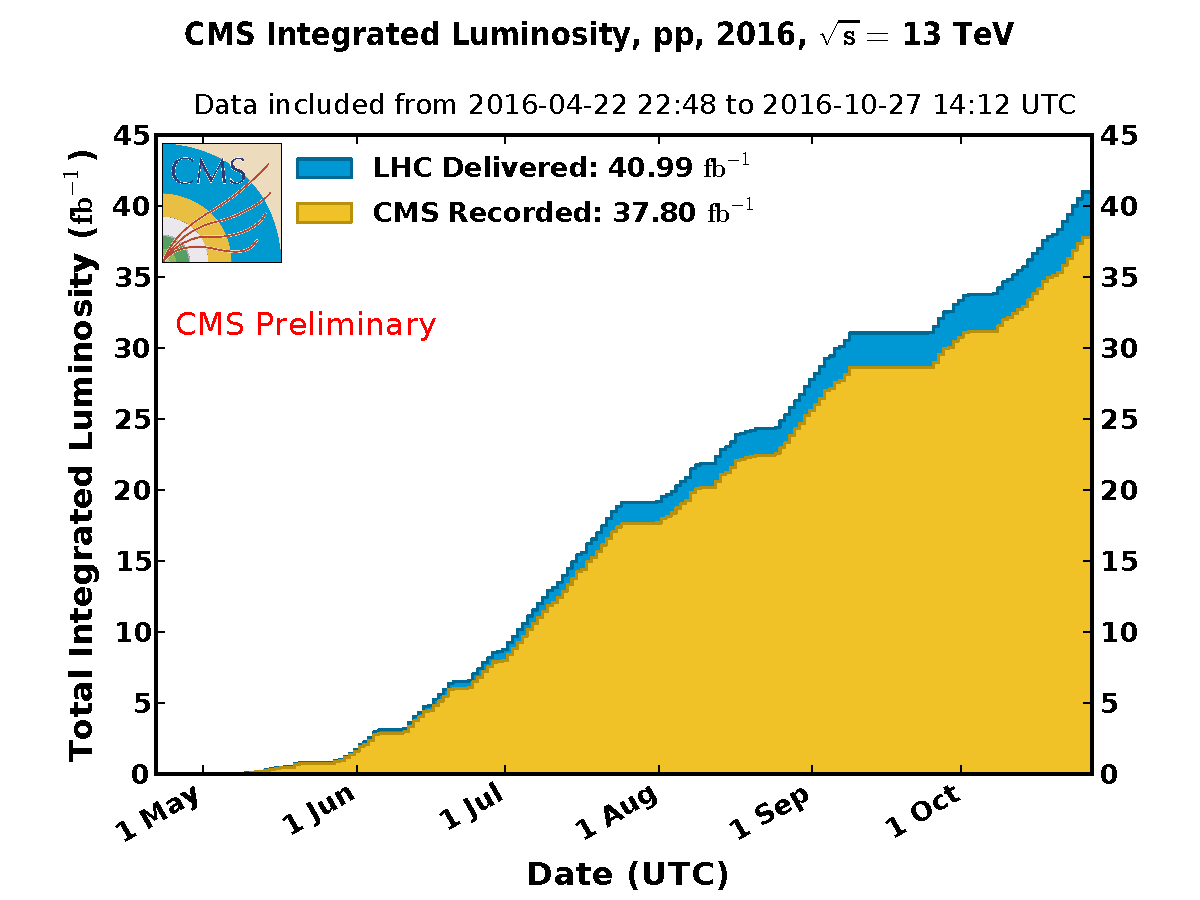
\includegraphics[width=0.7\linewidth]{../Figures/Chap2/int_lumi_per_day_cumulative_pp_2016}
\caption[Integrated luminosity of data]{Total integrated luminosity as delivered by LHC and recorded by CMS as a function of time}
\label{fig:int_lumi_per_day_cumulative_pp_2016}
\end{figure}
Total integrated luminosity (\lumi) as delivered by LHC and recorded by the CMS detector as a function of time is shown in Fig.~\ref{fig:int_lumi_per_day_cumulative_pp_2016} for the year 2016~\cite{lumicms}. The total data certified as good for physics analysis corresponds to $\lumi = 35.9\ \fbinv$.
\subsection{CMS coordinate system}
A right handed cartesian coordinate system adopted by the CMS has origin at the nominal collision point. The $x$-axis points towards inner side of the LHC ring, $y$ points upwards and $z$ axis is along the beam direction. The azimuthal angle $\phi$ is measured from $x$-axis in $x-y$ plane and $r$ is the radial distance. Psudorapidity is defined as $\eta = - \ln(\tan(\theta/2))$, where $\theta$ is the polar angle measured from $z$-axis. Psudorapidity is an approximation of rapidity variable defined as $\frac{1}{2}\ln((E+p_z)/(E-p_z))$ in the limit $E\approx |\textbf{p}|$, where E and \textbf{p} are energy and momentum respectively. Some of the other quantities which are used in this work are listed below.
\begin{align}
\mathrm{Transverse\ momentum,\ } p_T & = \sqrt{p_{x}^2 + p_{y}^2}\\
\mathrm{Distance\ in\ }\eta-\phi \ \mathrm{plane,}\ \Delta R & = \sqrt{(\Delta \eta)^2 + (\Delta \phi)^2}
\end{align}

\subsection{Superconducting magnet}
The 12.5 m long superconducting magnet in the CMS detector is made up of NbTi coil and capable of providing magnetic field up to 4 T (operated to provide 3.4 T). Some of the goals of LHC physics program is to have a good momentum resolution of muons and other charged particles, tag tau leptons and b-quark jets etc. The magnetic field plays a crucial role in measuring the momentum of charged particles by the tracker and and outer muon systems, and also in identifying the charge of particles. The magnetic flux returns through a 10 kilo-ton iron yoke. Total energy stored in the magnet is 2.6 GJ at 4 T magnetic field and the energy stored per unit cold mass is 11.6 kJ/kg which is higher than the values of any of the magnets used in particle physics detectors.
\subsection{Inner tracking system}
The tracking system is used to measure the momentum of the charged particles, determine their trajectory and to help in locating primary and secondary vertices. At a luminosity of $10^{34}\ cm^{-2}s^{-1}$, on an average 1000 particles pass through the tracker every 25 ns. Tracker uses about 200 m$^2$ of Si, has length of 5.8 m and diameter of 2.5 m and covers up to $|\eta| = 2.5$. 

It is composed of inner pixel detector consisting of 3 layers at radii 4.4 cm, 7.3 and 10.2 cm in the barrel region. The other component is the Si strip tracker which extends up to 1.1 m in barrel region with 10 layers in it. On either side of the barrel are the endcaps which have 2 disks in the pixel detector and 3 plus 9 disks in the strip tracker. There are in total 1440 modules in pixel detector with 66 million pixels; 15148 modules in strip tracker with 9.3 million strips. A part of cross sectional schematic view of the tracker \cite{Collaboration_2014} is shown in Fig.~\ref{fig:Tracker} with different modules namely: pixel, inner barrel (TIB), outer barrel (TOB), inner disks (TID) and endcaps (TEC). 

\begin{figure}[h!]
\centering
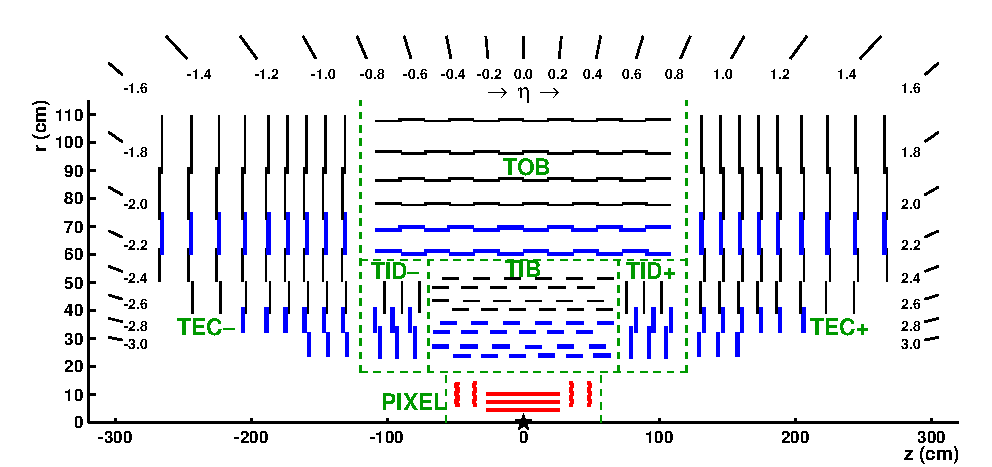
\includegraphics[width=0.95\linewidth]{../Figures/Chap2/Tracker}
\caption[CMS tracker]{A schematic view of the CMS tracker in $r-z$ plane showing different modules. The tracker is symmetric about $r=0$ line and the figure shows only the upper part.}
\label{fig:Tracker}
\end{figure}
The hit position resolution provided by the pixel detector is about 10 $\mu$m and 20-40 $\mu$m in transverse and longitudinal coordinate respectively and the third coordinate is determined from the sensor plane position.
\begin{table}[h!]
\centering
\caption[Characteristics of tracker]{Characteristics of subsystems of tracker. Pitch for the strip tracker refers to the distance between neighboring strips}
\label{tab:tracker}
\begin{tabular}{lllll}
\hline
Subsystem	&	Layers	&	Location (cm)	&	Pitch	&		Position resoln.\\\hline
Pixel barrel&	3 cylindrical	&	$r:$ 4.4 - 10.2 &	\multirow{2}{*}{$100\times150\ \mu m^2$}	&	$10\mu m$ in trans.\\
Pixel endcap&	2 disks	&		$z:$ 34.5 - 46.5	&		&	 $20-40\ \mu m$ longt.\\\hline
TIB			&	4 cylindrical & $r:$ 20 - 55 &	80 - 120 $\mu$m &	13 - 38 $\mu$m in $r\phi$\\\hline
TOB			&	6 cylindrical &	$r:$ 55 - 116&	122 - 183 $\mu$m &	18 - 47 $\mu$m in $r\phi$\\\hline
TID			&	3 disks		  &	$z:$ 58 - 124&	100 - 141 $\mu$m &	13 - 38 $\mu$m in $r\phi$\\\hline
TEC			&	9 disks		  &	$z:$ 124 - 282&	97 - 184 $\mu$m &	18 - 47 $\mu$m in $r\phi$\\\hline
\end{tabular}
\end{table}
The pixel and some of the strip modules (shown in thick blue lines in Fig.\ref{fig:Tracker}) are capable of providing 3-D hits and the strip modules which provide 2-D hits are shown in thin black line in the figure. The strip modules which provide 3-D hits consist of 2 back-to-back strips in them.

\subsubsection{Performance of tracker}
Figure \ref{fig:trackerResoln_muons} shows the resolution of various quantities for single muons of \pt 1, 10 and 100 \gev as a function of $|\eta|$.
\begin{figure}[h!]
\centering
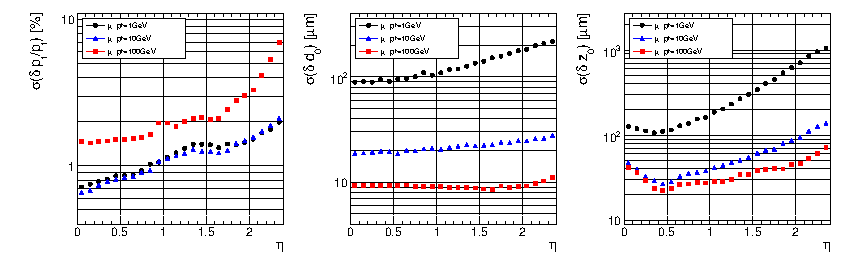
\includegraphics[width=0.98\linewidth]{../Figures/Chap2/trackerResoln_muons}
\caption[Tracker resolution for muons]{Resolution of various track parameters for muons with \pt = 1 \gev (black), 10 \gev (blue) and 100 \gev (red) . Left plot shows \pt resolution, middle plot shows transverse impact parameter resolution and right plot shows longitudinal impact parameter resolution.}
\label{fig:trackerResoln_muons}
\end{figure}
\begin{figure}[h!]
\centering
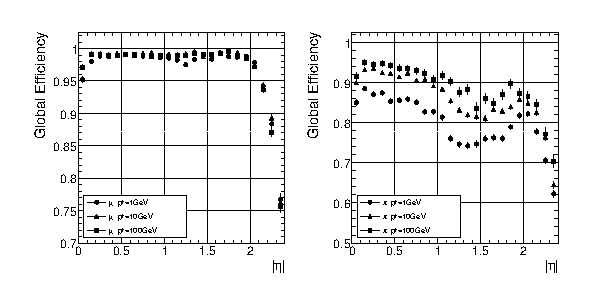
\includegraphics[width=0.98\linewidth]{../Figures/Chap2/trackerEff_muPions}
\caption[Track reconstruction efficiency]{Global track reconstruction efficiency for muons (left) and pion (right) with \pt of 1, 10 and 100 \gev.}
\label{fig:trackerEff_muPions}
\end{figure}

For 100 \gev muons, \pt resolution is about 1-2\% up to $|\eta| \approx 1.6$. For lower \pt muons, resolution mainly is affected by multiple scattering and for high \pt this effect is about 20-30\%. Multiple scattering of low \pt muons degrades the impact parameter resolution as well and this effect is reduced for high \pt muons and hence these have better impact parameter resolution.

Track reconstruction efficiency is about 99\% for muons with \pt in the range 1-100 \gev (left plot in Fig.\ref{fig:trackerEff_muPions}) and slight degradation for some $|\eta|$ regions is because of gaps or non-coverage of the tracker. For charged pions (right plot in Fig.\ref{fig:trackerEff_muPions}) the efficiency is lower because of interactions with the materials of the tracker. Thickness $t$ of the tracker in terms of radiation length, $X_0$ (left) and interaction length, $\lambda_I$ (right) is shown in Fig.\ref{fig:tracker_material} along with the supporting systems and beam pipe contributions using simulation. In an ideal case, the thickness of the tracker should be zero.

\begin{figure}[h!]
\centering
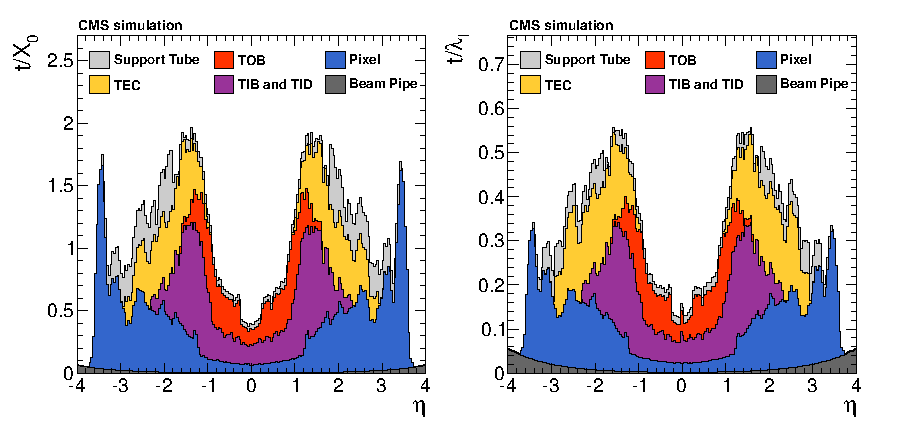
\includegraphics[width=0.98\linewidth]{../Figures/Chap2/tracker_material}
\caption[Tracker material budget]{Thickness of tracker along with beam pipe and supporting systems in terms of radiation length, $X_0$ (left) and interaction length, $\lambda_I$ (right).}
\label{fig:tracker_material}
\end{figure}

\subsection{Electromagnetic calorimeter}
The EM calorimeter (ECal) of CMS is a hermetic, compact, granular, homogeneous, radiation tolerant and total absorption calorimeter made up of lead tungstate crystals ($PbWO_4$). It measures energy of photons, electrons and EM component of jets. It has large dynamic range coupled with excellent linearity up to 1 TeV. It also provides triggering information and aids particle identification. The region with $|\eta| \leq 1.48$ is covered by barrel (EB) and $1.48 < |\eta| < 3$ region is covered by two endcap (EE) calorimeters. To identify neutral pions ($\pi^0$), a preshower (ES) detector is used in the endcaps with $1.653 < |\eta| < 2.6$. The radiation length of EB is $26X_0$, EE is $25X_0$ and that of ES is $3X_0$.

Incident electrons and photons produce EM showers which spread laterally over several crystals. Charged particles in these showers produce blue-green scintillation light (420-430 nm) and the amount of light is proportional to the incident particle energy. About 80\% of the scintillation light is emitted in 25 ns. The crystals have radiation length of 0.89 cm and small Molière radius (2.2 cm) which help in containment of shower in smaller volume. The scintillation light is collected by avalanche photo-diodes (APDs) in case of EB and vacuum photo-triodes (VPTs) in case of EE. 

Fig.\ref{fig:Ecal_sche_res} (left) shows the schematic layout of ECal modules, supermodules and supercrystals. The granularity of crystals in EB is $0.0174\times 0.0174$ in $\eta-\phi$. Two rows of 5 crystals form a submodule, A supermodule is formed using 4 modules. Almost all the crystal axes are tilted by 3\textdegree\ with respect to the line from nominal interaction point in both $\eta$ and $\phi$ directions to avoid any particle passing through the gap between crystals.
\begin{figure}[h!]
\centering
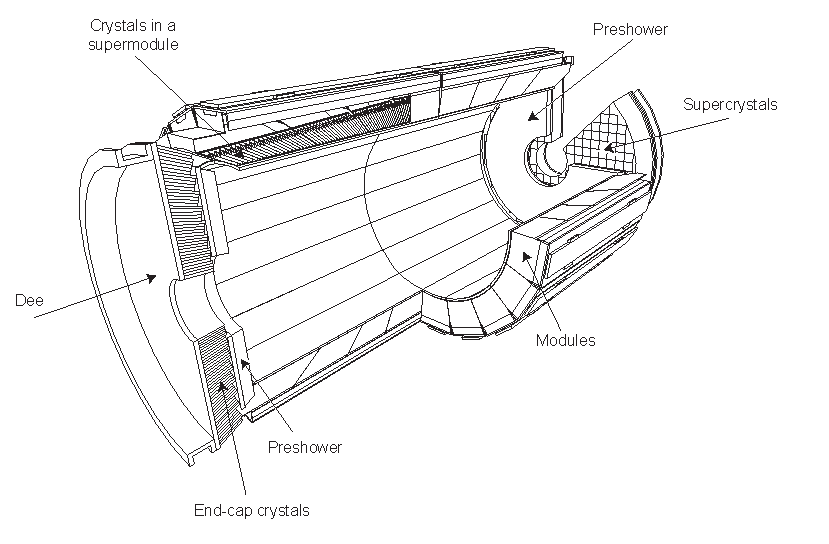
\includegraphics[width=0.59\linewidth]{../Figures/Chap2/Ecal_schematic}
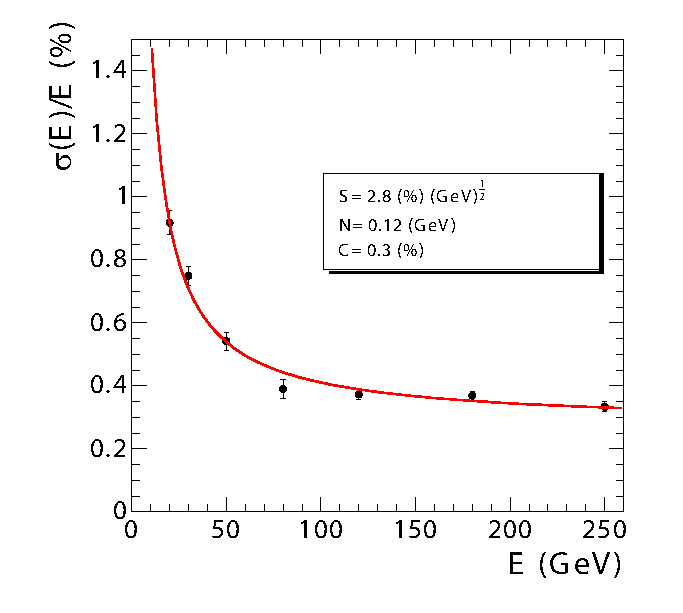
\includegraphics[width=0.4\linewidth]{../Figures/Chap2/ecalResolution}
\captionsetup{width=.95\linewidth}
\caption[ECal schematic and resolution]{A schematic of ECal showing different components is shown on the left. Right plot shows resolution of ECal as a function of electron energy using test beam studies.}
\label{fig:Ecal_sche_res}
\end{figure}

\noindent The energy resolution of ECal is given the expression,
\begin{equation}
\label{eqn:ecalReso}
{\left(\frac{\sigma}{E}\right)}^2  =  {\left(\frac{S}{\sqrt{E}}\right)}^2 + {\left(\frac{N}{E}\right)}^2 + C^2
\end{equation}
where $S$ is the stochastic term, $N$ is the noise term and $C$ is the constant term. Typical values after summing energy in $3\times3$ crystals are $S=2.8\%,\ N=0.12,\ C=0.3\%$. The resolution as a function of electron energy, $E$ measured in \gev is shown in Fig.\ref{fig:Ecal_sche_res} using test beam studies. The contributors of $S$ are shower fluctuations and photo-statistics; for $N$ the contributors are non-uniformity of longitudinal light collection, intercalibration errors and energy leakage; noise from electronics, digitization and pileup contribute to constant term.

A laser monitoring system is used to measure the transparency loss in the crystals which occurs because of radiation damage. This system uses blue laser of wavelength 440 nm which is closer to the scintillation peak and the intensity of the output light from each of the crystals is used to correct the transparency loss and re-calibrate the crystals.

\subsection{Hadron calorimeter}
This calorimeter (HCal) is a sampling calorimeter which measures energy of the hadrons and extends up to $|\eta| = 5.2$. It is divided into barrel (HB), endcap (HE), forward calorimeter (HF) and outer calorimeter (HO). 

The psudorapidity coverage of HB is $|\eta| < 1.3$ with a granularity width of 0.087 in both $\eta$ and $\phi$. This sampling calorimeter has alternating brass (70\% Cu and 30\% Zn) absorber and plastic scintillators. The absorber thickness is $5.82\lambda_I$ at 90\textdegree and $10.6\lambda_I$ at $|\eta| =1.3$. The ECal in front of HB has $1.1\lambda_I$. Fig.\ref{fig:Hcal_schematic} shows a schematic diagram of one quarter slice of HCal.
\begin{figure*}[h!]
\centering
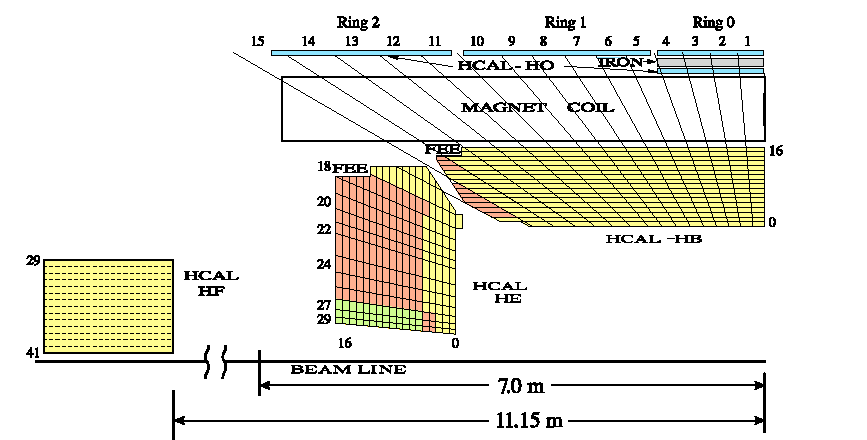
\includegraphics[width=0.9\linewidth]{../Figures/Chap2/Hcal_schematic}
\caption[Schematic diagram of HCal]{A schematic diagram of one quarter slice of HCal showing HB, HE, HO and HF along with location of front end electronics (FEE) of HB and HE. The colors represent longitudinal readout scheme.}
\label{fig:Hcal_schematic}
\end{figure*}
Because of space constraint from the magnet, HB thickness in the low $|\eta|$ region is kept small, and to record the leakage of hadronic showers, 5 rings of HO are placed outside the magnet. About 5\% of all hadrons of energy more than 100 \gev deposit energy in HO.

The scintillation light is collected by the wavelength shifting (WLS) optical fiber which is laid out on the edge of the scintillator tile. WLS fiber is spliced into clear fiber and the light is guided to hybrid photo-diode (HPD) using optical cable. HF uses Cherenkov based quartz fibers instead of scintillators and light from the quartz fibers is fed into photo-multiplier tubes (PMTs). More details about HF is discussed in later part of this chapter.

The signals from HPDs or PMTs are read by charge integration and encoding (QIE) chips. QIE is an ADC which provides almost constant precision over large range by assigning different number of bits to different amounts of charge (which is proportional to energy) collection.

All of the subsystems have LEDs and lasers for the purpose of calibration and monitoring. Except HO, other subsytems are also equipped with radioactive source tubes.

The resolution of HCAL and ECAL setup was determined using test beam setup and it found to be of the form:
\begin{equation}
\frac{\sigma}{E} = \frac{a}{\sqrt{E}} \oplus b
\end{equation}
where $a$ is stochastic term of value $0.847\pm 0.016\ {\mathrm{GeV}}^{\frac{1}{2}}$ and $b$ is a constant term of value $0.074\pm0.008$ for HB and HE. For HF, $a = 1.98 {\mathrm{GeV}}^{\frac{1}{2}}$ and $b = 0.09$ \cite{Collaboration_2010}.

A study on HF calorimeter performance in 2016 using energy deposits in HF quartz fibers is described in \ref{chap2HFsec}.

\subsection{Muon chambers}
Muons are detected using gas filled muon chambers located outside the magnet. The direction of magnetic field is opposite in direction to that of the field inside the magnet. The muon chambers have the task of identifying momentum of muons, type of charge and provide triggering information. This system consists of barrel region, up to $|\eta| = 1.2$, made up of drift tubes (DT) and two endcaps on either side, covering $0.9 < |\eta| < 2.4$, made up of cathode strip chambers (CSC). Restive plate chambers (RPSc) are mounted in both barrel and endcap and operated in avalanche mode. They are capable of providing excellent timing resolution needed for muon triggers and they cover $|\eta| < 1.9$. Fig.\ref{fig:Muon_chambers} shows a quarter of CMS detector with different muon chambers and their respective locations \cite{Sirunyan:2018fpa}.
\begin{figure}[h!]
\centering
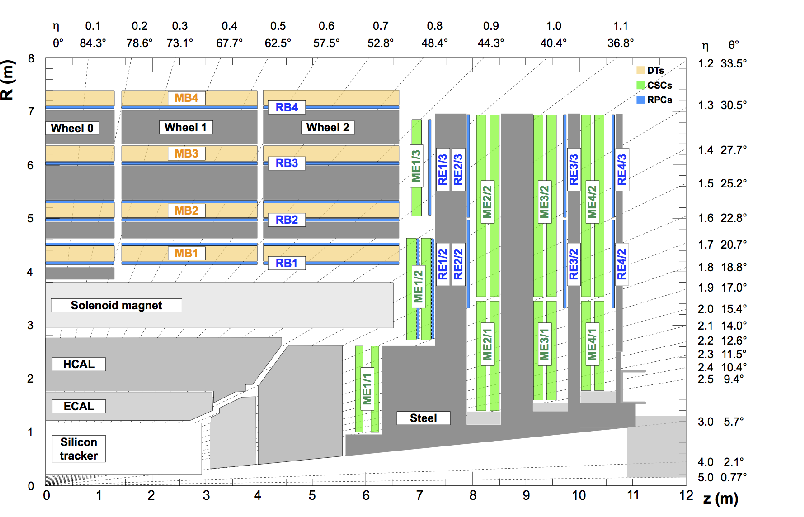
\includegraphics[width=0.95\linewidth]{../Figures/Chap2/Muon_chambers}
\captionsetup{width=.95\linewidth}
\caption[Muon chambers]{Schematic diagram of a quarter of CMS detector showing different components of muon chambers. Steel-flux return disks are shown as dark areas, DTs are labelled as MB, CSCs are labelled as ME, and RPCs are labelled as RB and RE. In this labelling $B$ refers to barrel and $E$ refers to endcap.}
\label{fig:Muon_chambers}
\end{figure}

As the muon passes through the chambers, it ionizes gas in these chambers. Each of the DTs chambers have drift cells of size $42\times 13$ mm$^2$ in transverse direction. The CSCs are operated as standard multi-wire proportional counters. More detailed description of muon system and its performance can be found in Ref.\cite{Sirunyan:2018fpa,Chatrchyan:2008aa,Chatrchyan:2013sba}.

The \pt resolution of muons is approximately 1\% in barrel and 3\% in endcap for $\pt < 100$ \gev \cite{Sirunyan:2018fpa}. The combined momentum measurement from tracker and muon system significantly improves the resolution and Fig.\ref{fig:muonPt_resoln} shows \pt resolution as a function of \pt of muon.

\begin{figure}[h!]
\centering
\includegraphics[width=0.8\linewidth]{../Figures/Chap2/muonPt_resoln}
\captionsetup{width=.95\linewidth}
\caption[Muon \pt resolution]{\pt resolution of muons as a function of \pt for $|\eta| < 0.8$ (left) and $1.2 < |\eta| < 2.4$ using tracker only, muon system only and combination of both \cite{Chatrchyan:2008aa}.}
\label{fig:muonPt_resoln}
\end{figure}


\section{Energy response in long and short fibers of HF calorimeter}
\label{chap2HFsec}
The HF is located at 11.3 m from the interaction point and provides a
pseudo-rapidity coverage from $|\eta|>3.0$ to $|\eta|<5.2$. Since
there is no coverage from the tracker or ECAL in this region, the energy deposited in HF
is used to reconstruct forward jets and also to calculate
\ptmiss. Hence a stable performance of HF is important both for SM
measurements and new physics searches.

The quartz fibers are inserted into the steel absorber plates. Half
of the fibers run over the full depth of the HF (165 cm $\approx$ 10
interaction lengths) while the remaining half of the fibers start at a
depth of 22 cm from the front face of the detector. The former
are called {\bf long fibers} and latter are called {\bf short
  fibers}. The energies deposited in long and short fibers are read
out separately, and are called {\elong} and {\eshort} respectively.

The signal in HF is due to the Cherenkov light produced by charged particles as they traverse through the quarts fibers. The
Cherenkov light is emitted only when the particle's velocity is greater than the speed of light in that medium. This light is collected by 
the long and short optical fibers. The recordable signal in calorimeter is due to the electromagnetic and hadronic component of the 
particle showers. Since electrons or photons result in shorter showers, these result in signal mostly
in long fibers. The hadronic showers, however, continue deeper and
result in signal in both long and short fibers.

The ratio of energy measured in short and long fibers,
\ratiosl = \eshort/\elong, depends on the energy of the incident
particle which created the shower and hence on how deeply the shower
has penetrated the calorimeter. However, the average \ratiosl
over a period of time in a given $\eta$ region is expected
to depend on average energy incident on the calorimeter and
accelerator run conditions (which determines the pileup, the number of pp interactions). In this
section, we describe studies \ratiosl for data collected at $\sqrt{s} = 8$
TeV and  $\sqrt{s} = 13$ TeV, and also the effect of pileup. 
Since the average \ratiosl for various channels of a
given $i\eta$ ring is expected to be same, this quantity is proposed to
be used to intercalibrate the short fibers across $\phi$
while the long fibers are calibrated using Z$\rightarrow e^+e^-$ events.

\subsection{Data and simulation samples}\label{sec:dataset}
These studies make use of data collected by CMS detector in the years 2012, 2015 and 2016.
Each of these are divided into different parts and they are named by adding a suffix to the year,
for example 2012D is a subset of data collected in 2012. The events from these dataset are selected
using triggers which are based on hadronic activity, calculated using sum \pt of all jets or using 
highest \pt jet in the event. The dataset which contains hadronic triggers is called as \textit{JetHT} dataset. 
Only those data which are certified as good for physics analysis are used. 
Table \ref{tab:dataSamples} shows list of datatsets used for this study along with pp bunch spacing and integrated 
luminosity of the dataset.
Monte-carlo (MC) simulated sample consists of QCD events generated at
leading order (LO) taking $\sqrt{s}=13$ TeV using MadGraph generator and hadronization is carried out using Pythia8.

\begin{table}[!h]
\centering
\caption[Collision data used for \ratiosl studies of HF]{Collision data used for \ratiosl studies of HF. The 2012 data were taken at $\sqrt{s}=8$ TeV and all other data were taken at $\sqrt{s}=13$ TeV.}
\label{tab:dataSamples}
\begin{tabular}{lccc}
\hline
Data	&	Bunch spacing (ns) 	& \lumi \ (\pbinv)\\\hline\hline
2012D	&	50					&	962 \\\hline
2015B	&	\multirow{2}{*}{50}	&	40.9\\
2015C	&						&	25.0\\ \hline
2015C	&	\multirow{2}{*}{25}	&	16.3\\
2015D	&						&	$1.61\times 10^3$\\\hline
2016B	&	\multirow{7}{*}{25}	&	$5.28\times 10^3$\\
2016C	&						&	$789$\\
2016D	&						&	$3.28\times 10^3$\\
2016E	&						&	$4.05\times 10^3$\\
2016F	&						&	$3.11\times 10^3$\\
2016G	&						&	$7.11\times 10^3$\\
2016H	&						&	$8.68\times 10^3$\\\hline
\end{tabular}
\end{table}

%\graphicspath{{/home/vinay/work/HFanalysisLocal/TreeMakerFiles/AnalysisNote/}}
\subsection{Energy in long and short fibers of HF}
The HF starts at $|\eta|$=2.853 and extends up to $|\eta|$=5.191. On 
both the $\pm z$ sides, this $\eta$ range is divided into 13 towers 
with tower index starting from $i\eta$=29 and ending at $i\eta$=41. 
Towers $|i\eta|$=29 to $|i\eta|$=39 have 36 divisions ($10^\circ$ each) 
in $\phi$ and towers $|i\eta|$=40 and 41 have 18 
divisions ($20^\circ$ each). In total there are 864 channels. Depth 
segment with index 1 corresponds to long fibers and depth segment
with index 2 refers to short fibers in each of these channels.
If the energy in a particular channel is above the noise level, then that channel is 
considered to have a \textit{rechit} (recorded hit).

All the plots and discussion till the end of section \ref{pileup} correspond to 2015C-50ns data.
\begin{itemize}
\item Fig.~\ref{fig:254833_ietavsIphiD1D2} shows a typical distribution of number of rechits, with rechit energy $>$ 10\,GeV, in each of the channels in depth 1 (long fibers) and depth 2 (short fibers). 
\begin{figure}[h!]
\begin{minipage}[b]{0.5\linewidth}
\centering
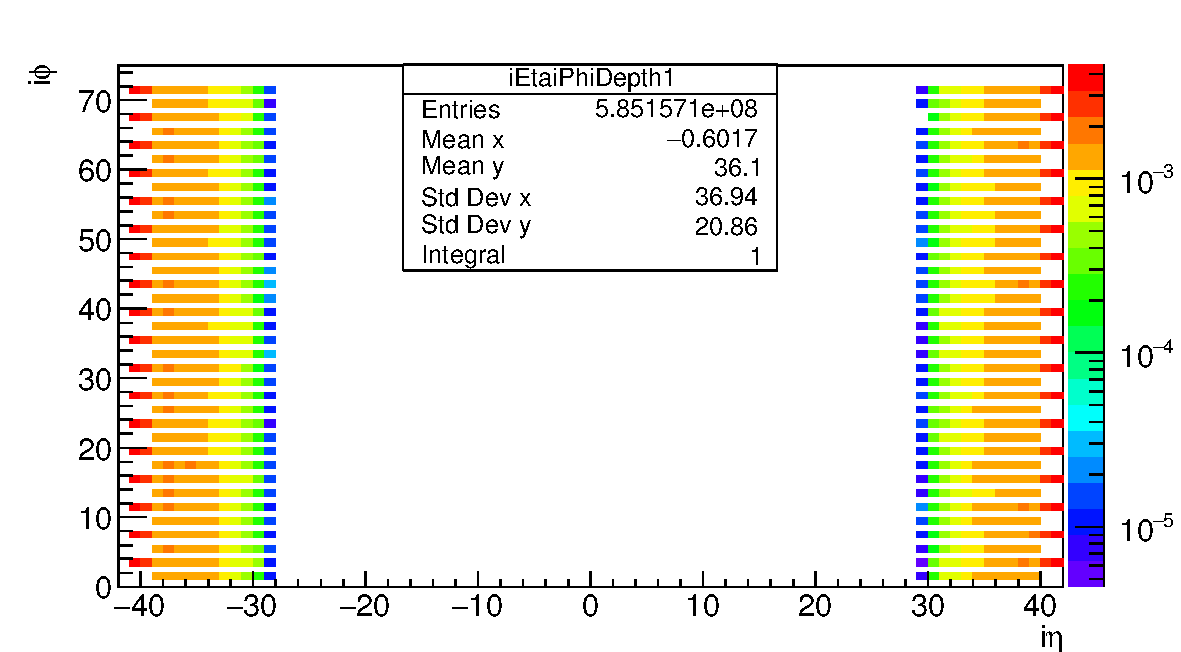
\includegraphics[width=.99\linewidth]{../Figures/Chap2/ImageFiles_HF/BasicPics/254833_ietavsIphiD1.pdf}
%\caption{Number of RecHits in depth 1}
%\label{fig:254833_ietavsIphiD1}
\end{minipage}
%\hspace{0.1cm}	
\begin{minipage}[b]{0.5\linewidth}
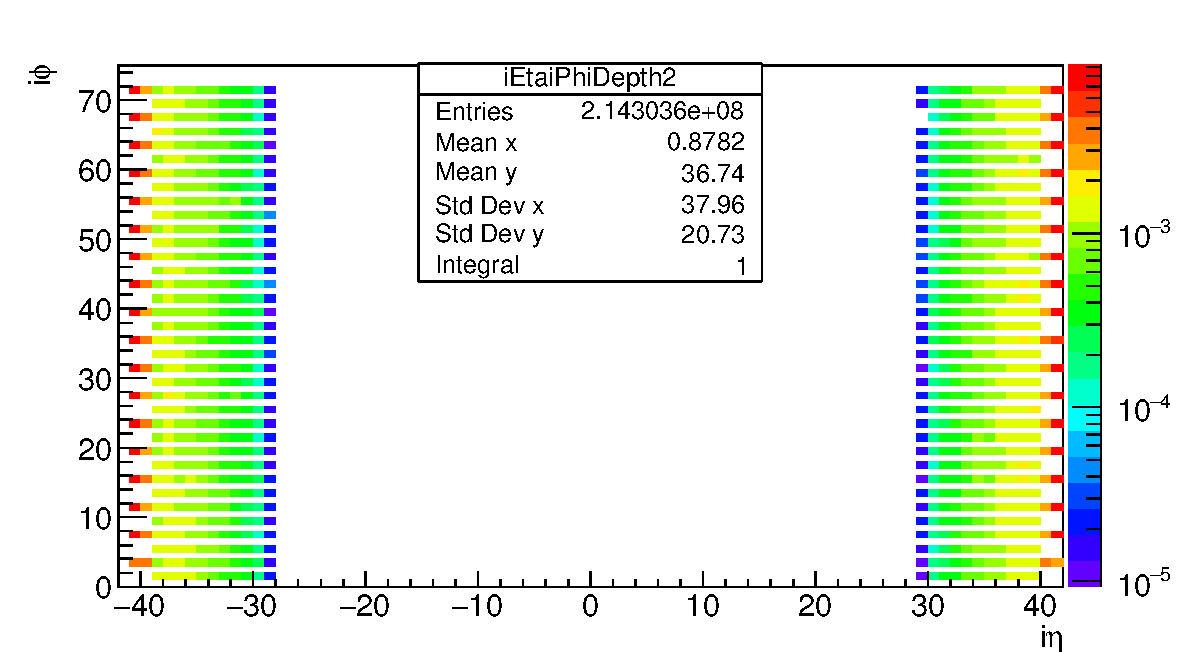
\includegraphics[width=0.99\linewidth]{../Figures/Chap2/ImageFiles_HF/BasicPics/254833_ietavsIphiD2.pdf}
%\caption{Channel occupancy for (left) depth 1, and (right) depth 2.}
%\label{fig:254833_ietavsIphiD1D2}
\end{minipage}
\caption[Channel occupancy for depth 1 and depth 2]{Channel occupancy for depth 1 (left), and depth 2 (right).}
\label{fig:254833_ietavsIphiD1D2}
\end{figure}

\item Fig.~\ref{fig:nRecHits} shows the total number of rechits 
distribution inclusive in $i\eta$ and $i\phi$ with rechit energy 
$>$10 GeV.
\begin{figure}[h!]
\centering
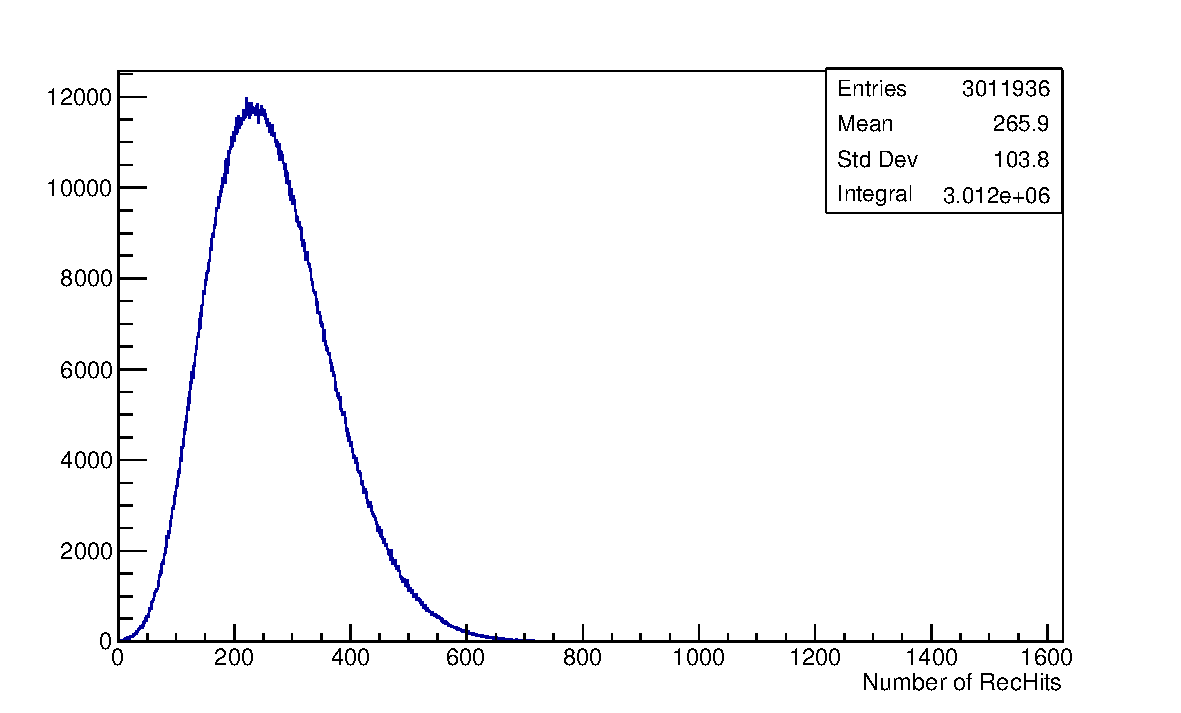
\includegraphics[width=0.5\linewidth]{../Figures/Chap2/ImageFiles_HF/BasicPics/nRecHits.pdf}
\caption{Total number of rechits (inclusive in $i\eta$ and $i\phi$) }
\label{fig:nRecHits}
\end{figure}
\item Fig.~\ref{fig:EsvsElNoECut} shows the energy distribution in 
short fibers (\eshort) vs long fiber (\elong) without any threshold
on their recorded energies. This figure shows that there is correlation 
between \elong and \eshort. So we use \ratiosl as a tool for studying 
the performance of HF.

There two more important points to note from this plot: firstly, there
are cases with a large \elong while there is almost no energy deposited 
in corresponding short fiber i.e. \eshort$<$ 10 GeV. This can be due to EM showers. Secondly, there are
cases when there is large energy deposited in short fibers while small
energies in long fibers (\elong$<$30 GeV). It is not expected to have 
large energy deposits in only one of the fibers if the shower originates
from hadrons. One of the reasons for this could be that some of the 
high energy particles directly hit the glass window of PMT and resultant Cherenkov light produced in the glass gives rise
to a large signal in only one of the channels. To reject such hits, 
thresholds are placed on reconstructed energies of rechits, \eshort$>10~$\gev
and \elong$>40~$\gev. From this point onwards, one can assume that these 
threshold have been applied on \eshort and \elong unless a different 
selection is explicitly mentioned.

\begin{figure}[h!]
\centering
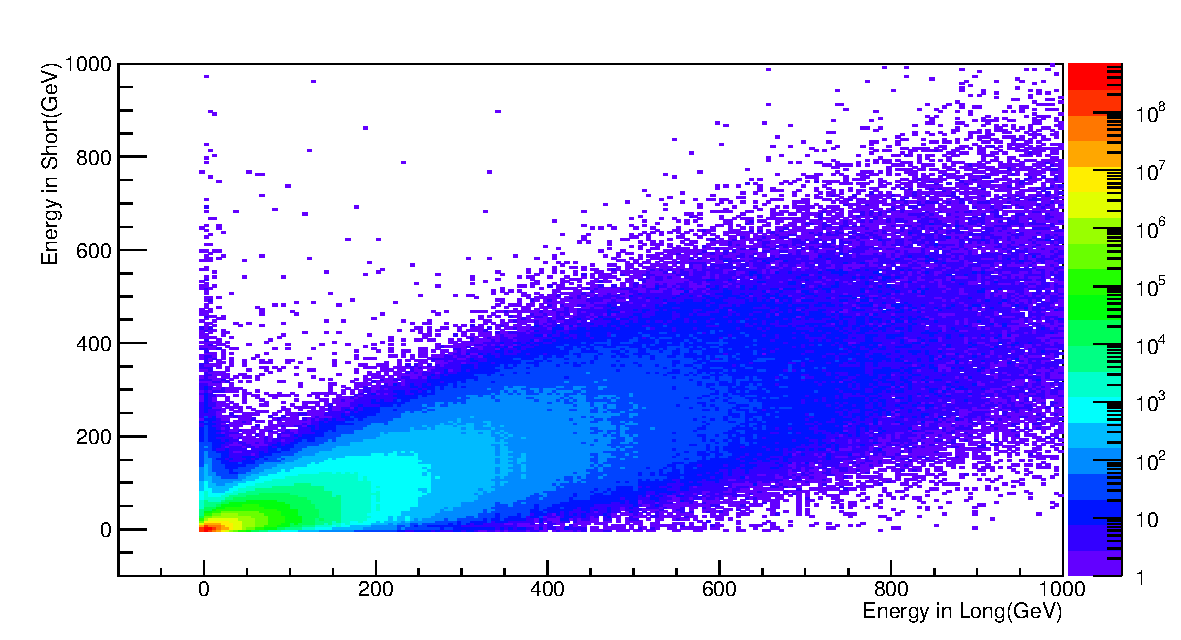
\includegraphics[width=0.7\linewidth]{../Figures/Chap2/ImageFiles_HF/BasicPics/EsvsElNoECut.pdf}
\caption{Distribution of \eshort vs \elong for HF channels.}
\label{fig:EsvsElNoECut}
\end{figure}

\item With the energy thresholds mentioned above, \ratiosl is studied 
for each $i\eta$ tower. Fig.\ref{1DRatio} shows distribution of
the \ratiosl for the tower $i\eta=$32 integrated over all $i \phi$ 
channels. Since the mean value of the distribution is sensitive to 
the tails, we try to fit it with an asymmetric Gaussian 
 (eqn.\ref{asymGaus}) and use the peak value obtained from the fit
to indicate the average ratio for a given $i\eta$ ring.

\begin{figure}[h!]
\centering
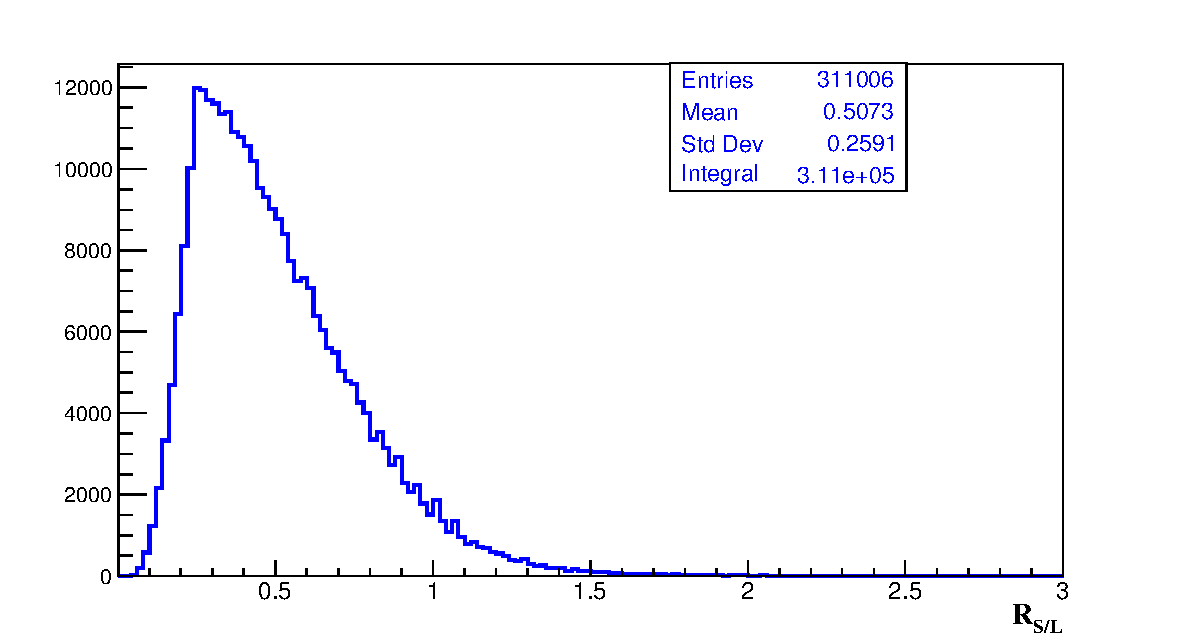
\includegraphics[width=0.7\linewidth]{../Figures/Chap2/ImageFiles_HF/Ratio/Ratioieta32254833El40.pdf}
\caption{\ratiosl for $i \eta\ 32$ tower with $i \phi$ inclusive for 2015D-50 ns.}
\label{1DRatio}
\end{figure}
\begin{equation}
f(x)=e^{-\frac{(x-\mu)^2}{2\sigma^2}}\left[ 1+erf\left( \frac{x-\mu}{\sqrt{2}\sigma}\right) \right] 
\label{asymGaus} 
\end{equation}
Fitting the \ratiosl with an asymmetric Gaussian works very well for 
smaller $i\eta$ channels (Fig.~\ref{goodfit}). For the channels in
higher $i\eta$ regions, fitting does not work well and $\chi^2/dof$ is 
very large (Fig.~\ref{badfit}). Changing the fit range did not improve the fits significantly. So using the peak obtained from the 
fits cannot be used for studying all the channels. We then use 90\% 
truncated mean of the distribution - starting from the arithmetic peak,
bin contents are added on both the sides until the total integral is
90\% of the total area under the curve. From this point onward, mean 
refers to 90\% truncated mean. 
%\textcolor{red}{Comparison between arithmetic mean, 
%truncated mean and the peak obtained from the fit for different 
%$i\eta$ are shown in appendix~\ref{AppendixA} Fig.~\ref{MeanvsFit}.
%Fits for all the $i\eta$ towers are shown in appendix~\ref{AppendixA}
%Figs.~\ref{fig:Ratioieta29to32} to \ref{fig:Ratioieta41}.}

\begin{figure}[ht]
\begin{minipage}[b]{0.45\linewidth}
\centering
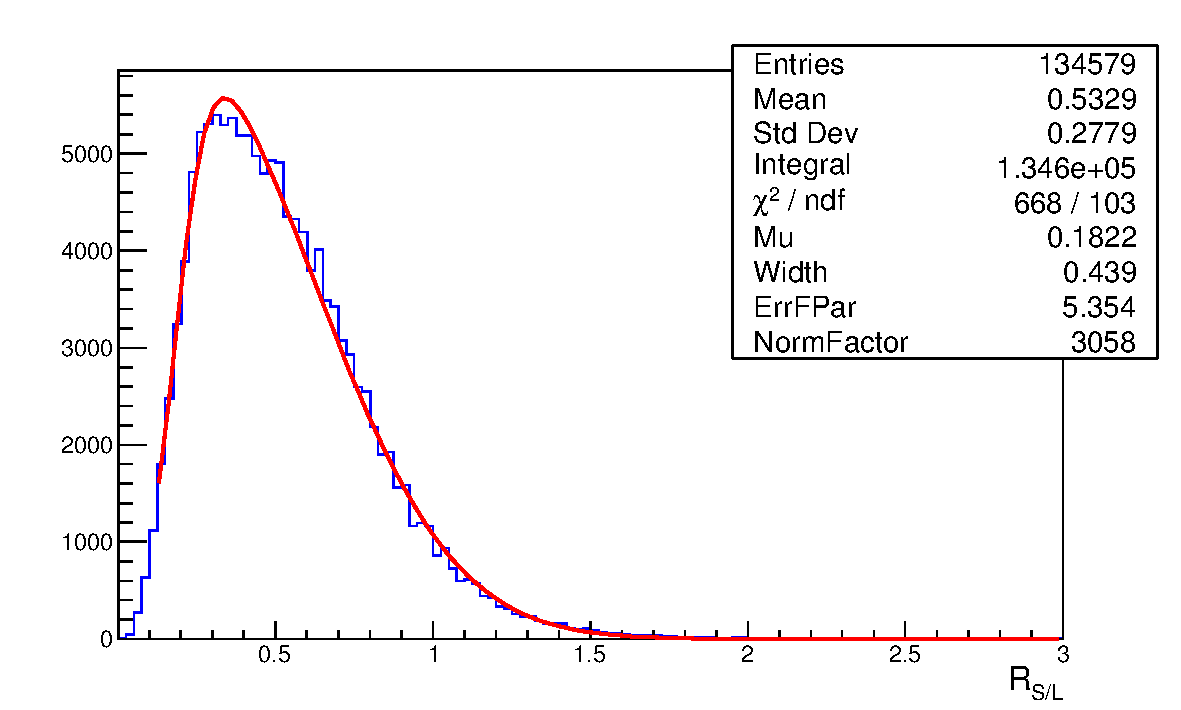
\includegraphics[width=\textwidth]{../Figures/Chap2/ImageFiles_HF/Ratio/RatioietaP30.pdf}
\captionsetup{width=.9\linewidth}
\caption{Asymmetric Gaussian fit for $i \eta$ 30}
\label{goodfit}
\end{minipage}
\hspace{0.5cm}
\begin{minipage}[b]{0.45\linewidth}
\centering
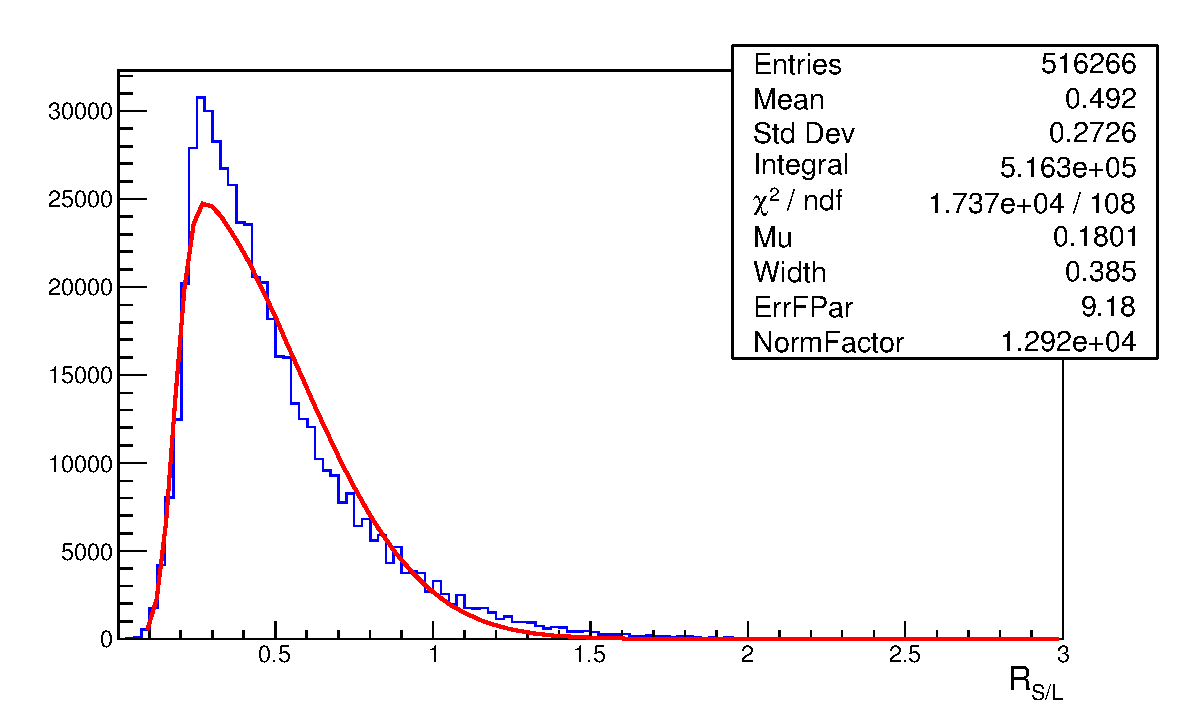
\includegraphics[width=\textwidth]{../Figures/Chap2/ImageFiles_HF/Ratio/RatioietaP39.pdf}
\captionsetup{width=.9\linewidth}
\caption{Asymmetric Gaussian fit for $i \eta$ 39}
\label{badfit}
\end{minipage}
\end{figure}

\subsection{Effect of Pileup on \ratiosl}\label{pileup}
The \ratiosl was studied under different pileup (PU) scenarios. If the number 
of good primary vertices is less than 9, it is considered as low pileup; 
between 11 and 16 as medium pileup and above 18 as high pileup.\\
Pileup is mainly dominated by low energy particles
and these particles do not have enough energy to penetrate into the short fibers and hence they deposit energy mainly in long fibers.
Hence these particles give lower \ratiosl than the high energy particles. Pileup is added on top of
a hard scattered events, and in hard scattered event \ratiosl is higher than PU events. Thus 
with increase of more and more pileup events, the \ratiosl is decreasing and that is the observation. With the high pileup, average energy deposits in long fibers is expected 
to be higher and as a result the \ratiosl is expected to be lower as 
compared to the low pileup scenario.Fig.~\ref{RvsIetaComparePileups} shows 
that higher pileup means lower ratio and lower pileup means higher ratio. 
The shaded region corresponds to all events wherein no restriction on pileup is 
applied.

\begin{figure}[h!]
\centering
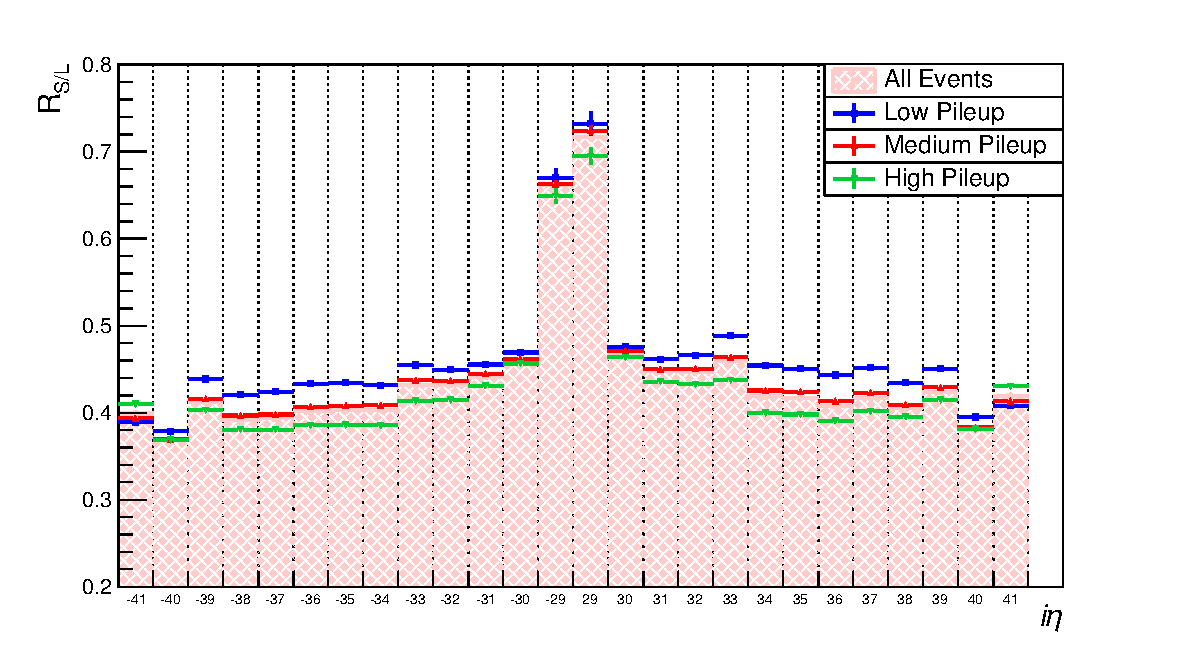
\includegraphics[width=0.7\linewidth]{../Figures/Chap2/ImageFiles_HF/Ratio/RvsIetaComparePileups.pdf}
\captionsetup{width=.9\linewidth}
\caption[Effect of pileup on \ratiosl for different $i\eta$]{Effect of pileup on \ratiosl for different $i\eta$ rings (integrated over $i\phi$ channels.}
\label{RvsIetaComparePileups}
\end{figure}

\end{itemize}


\subsection{Studying \ratiosl at $\sqrt{s}=$13 TeV and 8 TeV data with 50 ns bunch spacing}\label{sec:ana50ns}

\begin{itemize}
\item In 2015, LHC started 13 TeV collisions with 50 ns bunch spacing. We compared \ratiosl for 13 TeV data taken in 2015 and 8 TeV data taken in 2012.
\item Used JetHT dataset for 13TeV data and 8 TeV with all the events (no trigger based selection of events) for this study.
\item Average pile up was similar (Fig.\ref{fig:nVertices}) in 8 and 13 TeV datasets.

\begin{figure}[h!]
\centering
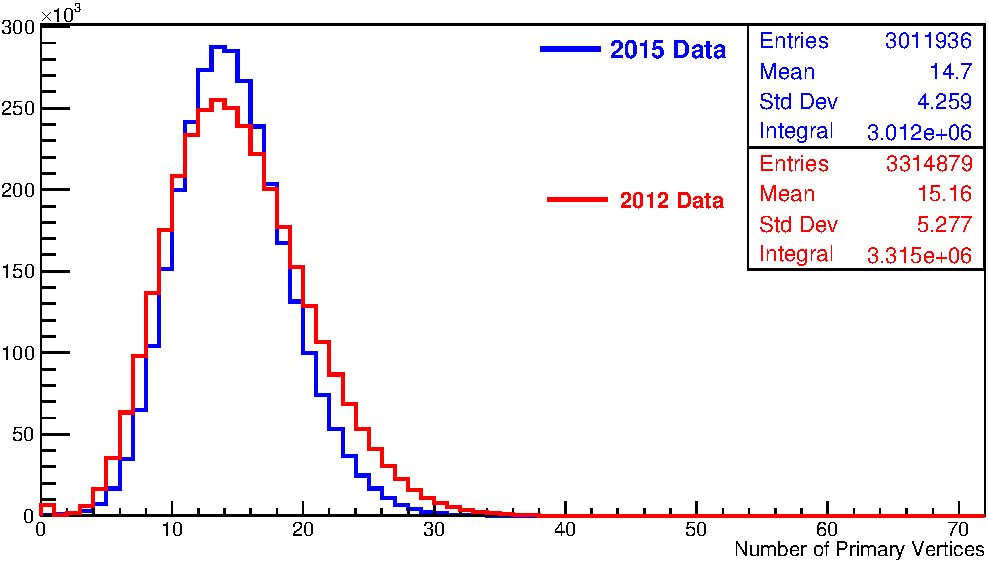
\includegraphics[width=0.7\linewidth]{../Figures/Chap2/ImageFiles_HF/2012vs2015/nVertices.pdf}
\caption{Pileup comparison for 2015 data and 2012 data}
\label{fig:nVertices}
\end{figure}

\item Fig.~\ref{2012vs2015E1} and \ref{2012vs2015E2} show the distributions of energies in long and short fibers, for 2012D and 2015C, with \elong, \eshort $>10~$\gev.

\begin{figure}[ht]
\begin{minipage}[b]{0.5\linewidth}
\centering
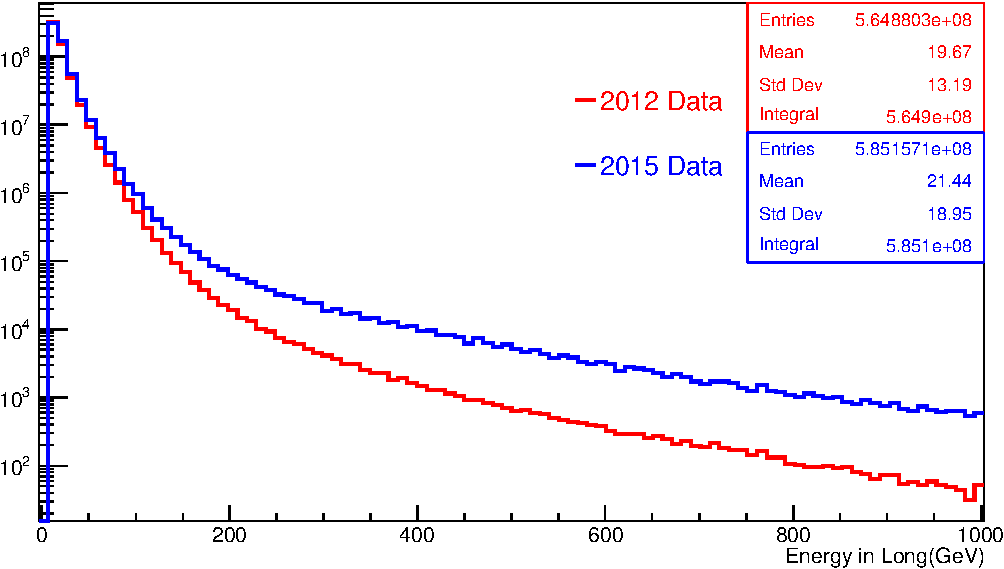
\includegraphics[width=\linewidth]{../Figures/Chap2/ImageFiles_HF/2012vs2015/Elong1DCompare.pdf}
\captionsetup{width=.9\linewidth}
\caption[\elong for 2012 and 2015 data]{Energy in long fibers for 2012 and 2015 data}
\label{2012vs2015E1}
\end{minipage}
\hspace{0.5cm}
\begin{minipage}[b]{0.5\linewidth}
\centering
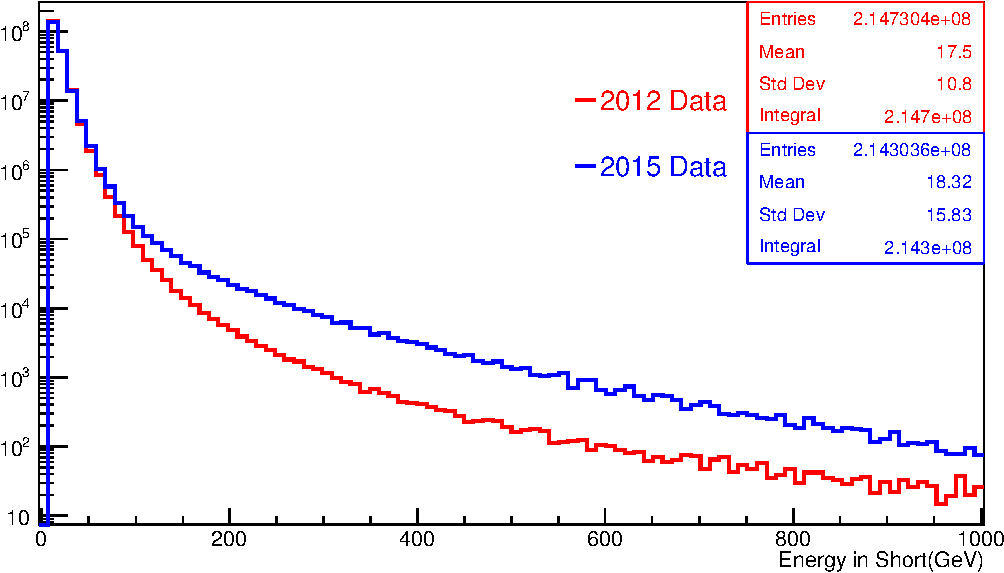
\includegraphics[width=\linewidth]{../Figures/Chap2/ImageFiles_HF/2012vs2015/Eshort1DCompare.pdf}
\captionsetup{width=.9\linewidth}
\caption[\eshort for 2012 and 2015 data]{Energy in short fibers for 2012 and 2015 data}
\label{2012vs2015E2}
\end{minipage}
\end{figure}
\end{itemize}

In 2015 p-p collisions, the $\sqrt{s}$ was 13 TeV and in 2012 it was only 8 TeV. 
Because of the increased energy of the collisions, the outgoing particles will have 
higher energy and hence these particles can penetrate deeper into the calorimeter giving
larger energy in short fibers. So the \ratiosl is expected to be higher in 13 TeV data as
compared to 8 TeV data. \ratiosl was determined for different $i \eta$ towers,with $i \phi$ 
inclusive and it was compared for 2012D data, 2015B data and 2015C data (fig, \ref{RvsIeta}).
For most of the $i \eta$ towers, \ratiosl of 2015 data is higher than that of 2012. With the 
increase of $\sqrt{s}$, average energy of particles is also increasing, consequently the 
\ratiosl is increasing. The reason for differences in 2015 and 2012 data could be because
of increased beam energy in p-p collisions and (or) the response of the fibers has changed.
\ratiosl for $|i\eta|$ 29 is much higher as compared to other $|i\eta|$ towers. This is because, this tower is behind $|i\eta|$ 28 of HE. EM shower energy is already deposited in HE. HF receives only hadronic shower energy and this energy is deposited in both long and short. Hence \ratiosl is higher for these towers.
\begin{figure}[h!]
\centering
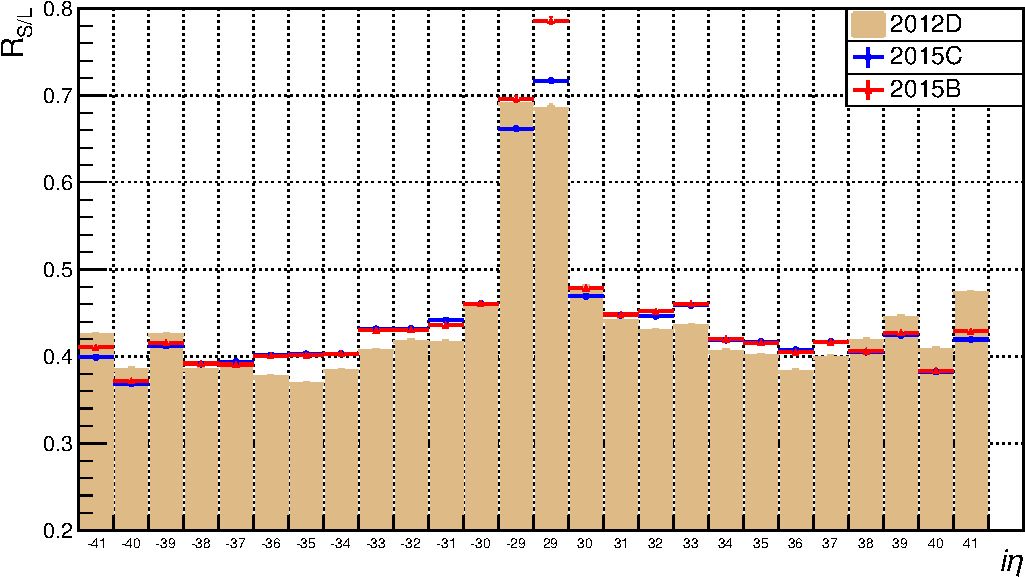
\includegraphics[width=0.7\linewidth]{../Figures/Chap2/ImageFiles_HF/2012vs2015/RvsIeta.pdf}
\caption{\ratiosl vs $i \eta$ for 3 different run conditions}
\label{RvsIeta}
\end{figure}
\ratiosl as a function of $i\phi$ for each $i \eta$ was also studied. Fig.~\ref{fig:Rvsiphi1} shows \ratiosl vs $i \phi$ for $i \eta$ -35. From this plot one can see whether a particular channel is problematic or not. In this figure, channel with $i \phi$ index 35 shows very high ratio in 2015B run. Also in most of the $i \phi s$, \ratiosl for 2012 data is slightly lower than 2015 data \ratiosl. %\textcolor{red}{The plots corresponding to each $i \eta$ is shown in Fig.\ref{fig:ieta29_32_E1E2Cut2Ietaiphi}-\ref{fig:ieta41E1E2Cut2Ietaiphi}  in appendix \ref{AppendixA}.}
\begin{figure}[h!]
\centering
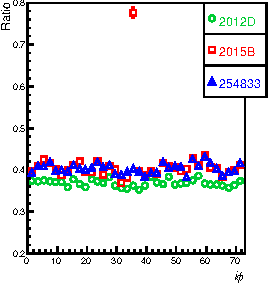
\includegraphics[width=0.5\linewidth]{../Figures/Chap2/ImageFiles_HF/2012vs2015/Rvsiphi1.pdf}
\caption{\ratiosl vs $i \phi$ plot for $i \eta$ -35}
\label{fig:Rvsiphi1}
\end{figure}



\subsection{\ratiosl for 2015 Data and 2016 Data}\label{sec:2015vs2016}
Data taken in 2015 with 25ns bunch spacing was compared with the 2016 data (25ns bunch spacing) using JetHT dataset and requiring at least one jet with \pt $> 450$ \gev at trigger level. This comparison is useful to understand the problems or changes in 2016 in HF, if any, with respect to the previous data taking.\\
Pileup conditions for 2015 and 2016B were different (Fig.\ref{nVtx2015D_2016B}). As discussed in sec.\ref{pileup}, if the pileup is high, then the \ratiosl is expected to be smaller since more energy goes into the long fibers.
\begin{figure}[ht]
\begin{minipage}[b]{0.5\linewidth}
\centering
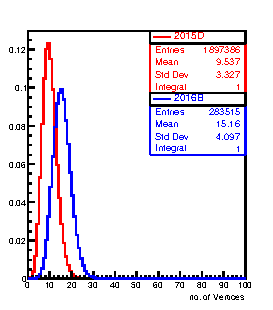
\includegraphics[width=0.99\linewidth]{../Figures/Chap2/ImageFiles_HF/BasicPics/Comp2015vs2016B/nVtx2015D_2016B.pdf}
\captionsetup{width=.9\linewidth}
\caption{Number of primary vertices before re-weighting}
\label{nVtx2015D_2016B}
\end{minipage}
\hspace{0.5cm}
\begin{minipage}[b]{0.5\linewidth}
\centering
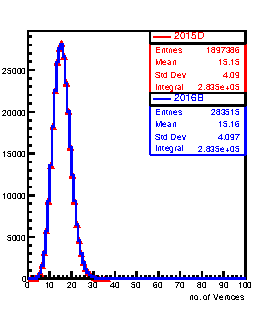
\includegraphics[width=0.99\linewidth]{../Figures/Chap2/ImageFiles_HF/BasicPics/Comp2015vs2016B/nVtx2015DPUwt_2016B.pdf}
\captionsetup{width=.9\linewidth}
\caption{Number of primary vertices after re-weighting}
\label{nVtx2015DPUwt_2016B}
\end{minipage}
\end{figure}

In order to compare the data taken with these different conditions, events had to be rewighted according to the pileup. In this case, number of primary vertices (PV) distribution in 2015D was re-weighted to match PV distribution of 2016B. This was done by simple division of 2016B histogram by 2015D histogram. The resulting histogram gives the pileup weights for 2015D as a function of different PVs. Fig.~\ref{nVtx2015DPUwt_2016B} shows the PV distribution after the reweighing. 
In Fig.~(\ref{nRecHits_2015DPUwt_2016B}-\ref{RecHitES_2015DPUwt_2016B}) some of the HF parameters such as number of RecHits above 10~GeV, RecHit energy in long and short fibers for these runs are compared. These runs show very similar behavior with respect to these parameters.
\begin{figure}[!h]
\begin{minipage}[b]{0.48\linewidth}
\centering
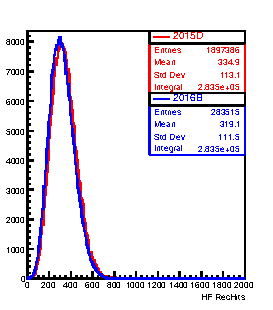
\includegraphics[width=0.9\linewidth]{../Figures/Chap2/ImageFiles_HF/BasicPics/Comp2015vs2016B/nRecHits_2015DPUwt_2016B.pdf}
\captionsetup{width=.9\linewidth}
\caption{No. of HF RecHits above 10 GeV}
\label{nRecHits_2015DPUwt_2016B}
\end{minipage}
%\hspace{0.5cm}
\begin{minipage}[b]{0.48\linewidth}
\centering
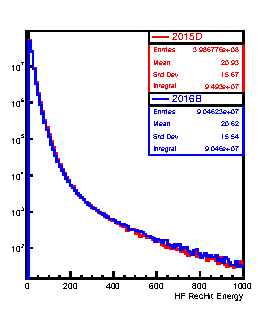
\includegraphics[width=0.9\linewidth]{../Figures/Chap2/ImageFiles_HF/BasicPics/Comp2015vs2016B/RecHitE_2015DPUwt_2016B.pdf}
\captionsetup{width=.9\linewidth}
\caption{HF RecHit energy in long and short fibers}
\label{RecHitE_2015DPUwt_2016B}
\end{minipage}
\end{figure}
\begin{figure}[!h]
\begin{minipage}[b]{0.48\linewidth}
\centering
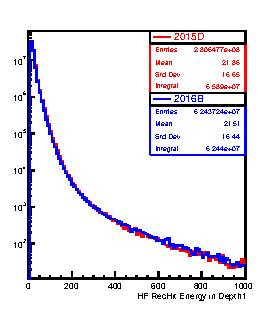
\includegraphics[width=0.99\linewidth]{../Figures/Chap2/ImageFiles_HF/BasicPics/Comp2015vs2016B/RecHitEL_2015DPUwt_2016B.pdf}
\captionsetup{width=.9\linewidth}
\caption{Energy in long}
\label{RecHitEL_2015DPUwt_2016B}
\end{minipage}
%\hspace{1cm}
\begin{minipage}[b]{0.48\linewidth}
\centering
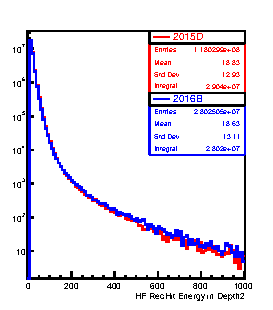
\includegraphics[width=0.99\linewidth]{../Figures/Chap2/ImageFiles_HF/BasicPics/Comp2015vs2016B/RecHitES_2015DPUwt_2016B.pdf}
\captionsetup{width=.9\linewidth}
\caption{Energy in short}
\label{RecHitES_2015DPUwt_2016B}
\end{minipage}
\end{figure}

\ratiosl as a function of different $i\eta$ for 2015 data and 2016B data are compared in Fig.\ref{fig:Ratio2015vs2015B}. The plot shows that both the datasets have similar ratio and the agreement between these datasets is within 1-2\%. It was found that the choice of a different hardonic trigger does not affect \ratiosl features seen in this plot.
\begin{figure}[h!]
\centering
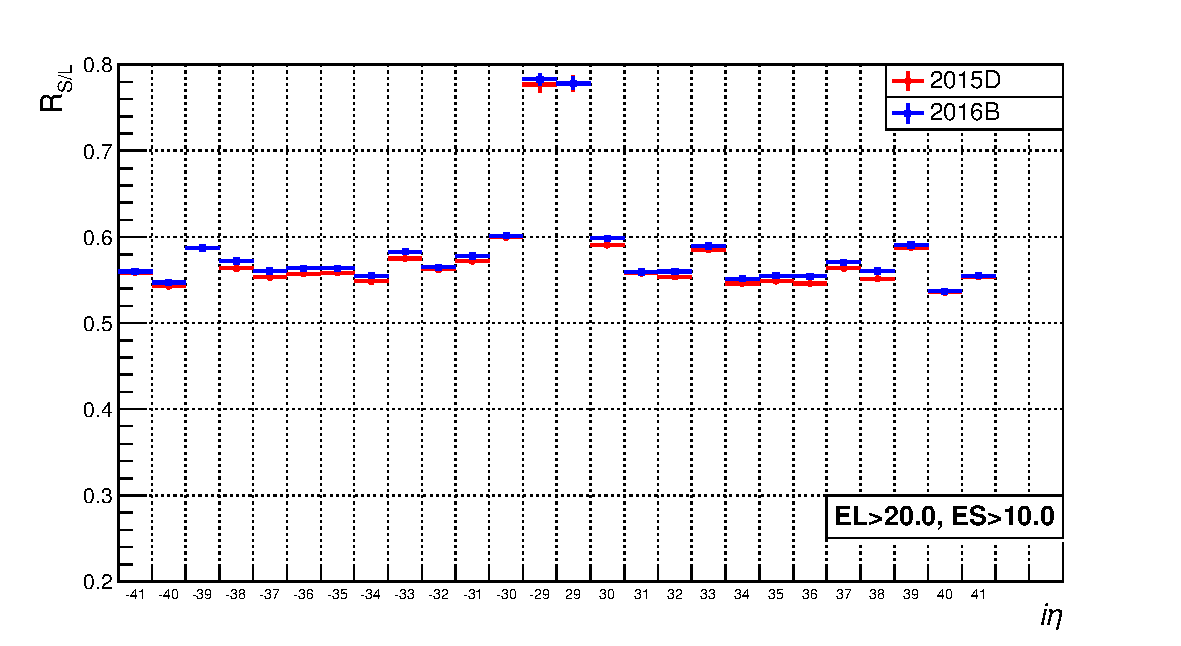
\includegraphics[width=0.7\linewidth]{../Figures/Chap2/ImageFiles_HF/Ratio/2015vs2016/Ratio2015vs2015B}
\caption{\ratiosl for 2015 and 2016B data}
\label{fig:Ratio2015vs2015B}
\end{figure}

\subsection{Performance of \ratiosl in 2016 Data}
In this section, different run eras of 2016 data (era B to H) are compared using JetHT dataset and events with 
at least one jet with $\pt > 450$ \gev at trigger level.
Different run eras of 2016 had different pileup scenarios and 2016B has the 
smallest pileup among these. This can be clearly seen from the distributions 
of number of primary vertices (Fig.~\ref{nVtx2016BtoH}).
 If the pileup is higher, then the number of rechits 
are also higher. So larger pileup runs have higher mean number of rechits as 
shown in Fig.~\ref{nRecHits2016BtoH}. All these distributions are
normalized to unit area.


\begin{figure}[!h] % nVtx2016BtoE and nVtx2016BFGH
%\begin{minipage}[b]{0.5\linewidth} % nVtx2016Bto
\centering
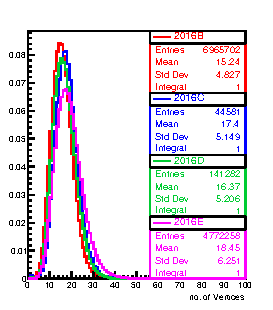
\includegraphics[width=0.45\linewidth]{../Figures/Chap2/ImageFiles_HF/BasicPics/Comp2016/nVtx2016BtoE.pdf}
%\caption{Number of PVs for 2016B,C,D,E}
%\label{nVtx2016BtoE}
%\end{minipage}
%\begin{minipage}[b]{0.5\linewidth} % nVtx2016BFGH
%\centering
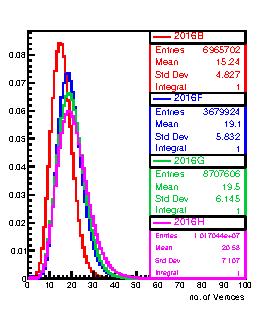
\includegraphics[width=0.45\linewidth]{../Figures/Chap2/ImageFiles_HF/BasicPics/Comp2016/nVtx2016BFGH.pdf}
\caption[No. of primary vertices for 2016 run eras]{Number of primary vertices (left) for 2016B,C,D,E, and (right) for 2016B,F,G,H.}
\label{nVtx2016BtoH}
%\end{minipage}
\end{figure}

\begin{figure}[!h] %nRecHits2016BtoE and nRecHits2016BFGH
%\begin{minipage}[c]{0.5\linewidth}
\centering
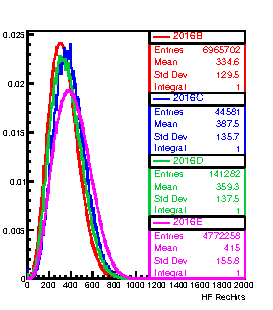
\includegraphics[width=0.45\linewidth]{../Figures/Chap2/ImageFiles_HF/BasicPics/Comp2016/nRecHits2016BtoE.pdf}
%\caption{Number of RecHits for 2016B,C,D,E}
%\label{nRecHits2016BtoE}
%\end{minipage}
%\begin{minipage}[c]{0.5\linewidth}
%\centering
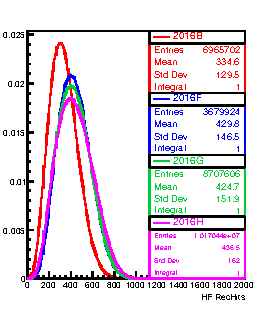
\includegraphics[width=0.45\linewidth]{../Figures/Chap2/ImageFiles_HF/BasicPics/Comp2016/nRecHits2016BFGH.pdf}
\caption[No. of rechits for 2016 run eras]{Number of RecHits (left) for 2016B,C,D,E, and (right) for 2016B,F,G,H.}
\label{nRecHits2016BtoH}
%\end{minipage}
\end{figure}

\begin{figure}[!h] %RecHit Energy 2016BtoE
\begin{minipage}[c]{0.32\linewidth}
\centering
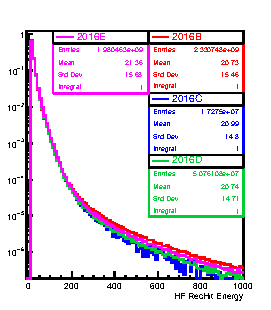
\includegraphics[width=0.99\linewidth]{../Figures/Chap2/ImageFiles_HF/BasicPics/Comp2016/RecHitsE2016BtoE.pdf}
%\caption{RecHitEnergy for 2016B,C,D,E}
%\label{RecHitsE2016BtoE}
\end{minipage}
\begin{minipage}[c]{0.32\linewidth}
\centering
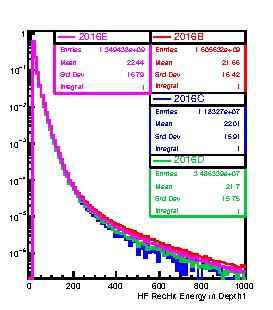
\includegraphics[width=0.99\linewidth]{../Figures/Chap2/ImageFiles_HF/BasicPics/Comp2016/RecHitsEL2016BtoE.pdf}
%\caption{RecHitEnergy in Long}
%\label{RecHitsEL2016BtoE}
\end{minipage}
\begin{minipage}[c]{0.32\linewidth}
\centering
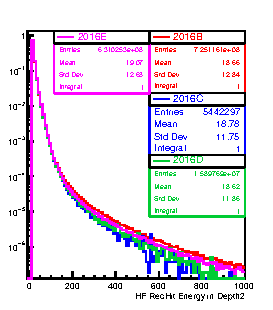
\includegraphics[width=0.99\linewidth]{../Figures/Chap2/ImageFiles_HF/BasicPics/Comp2016/RecHitsES2016BtoE.pdf}
%\caption{RecHitEnergy in Short}
%\label{RecHitsES2016BtoE}
\end{minipage}
\caption{RecHitEnergy distributions for 2016B,C,D,E}
\label{RecHitE2016BtoE}
\end{figure}
\begin{figure}[!h] %RecHit Energy 2016BFGH
\begin{minipage}[c]{0.32\linewidth}
\centering
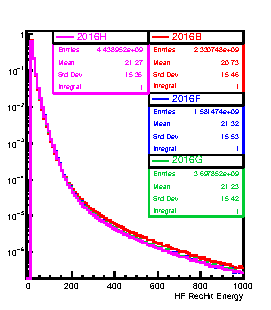
\includegraphics[width=0.99\linewidth]{../Figures/Chap2/ImageFiles_HF/BasicPics/Comp2016/RecHitsE2016BFGH.pdf}
%\caption{RecHitEnergy for 2016B,F,G,H}
%\label{RecHitsE2016BFGH}
\end{minipage}
\begin{minipage}[c]{0.32\linewidth}
\centering
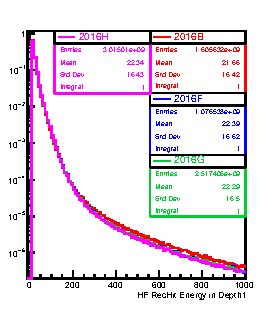
\includegraphics[width=0.99\linewidth]{../Figures/Chap2/ImageFiles_HF/BasicPics/Comp2016/RecHitsEL2016BFGH.pdf}
%\caption{RecHitEnergy in Long}
%\label{RecHitsEL2016BFGH}
\end{minipage}
\begin{minipage}[c]{0.32\linewidth}
\centering
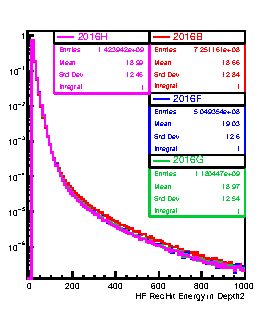
\includegraphics[width=0.99\linewidth]{../Figures/Chap2/ImageFiles_HF/BasicPics/Comp2016/RecHitsES2016BFGH.pdf}
%\caption{RecHitEnergy in Short}
%\label{RecHitsES2016BFGH}
\end{minipage}
\caption{RecHitEnergy distributions for 2016B,F,G, H}
\label{RecHitE2016BFGH}
\end{figure}
RecHit energy distributions for all run eras of 2016 show similar features (Fig.\ref{RecHitE2016BtoE} - \ref{RecHitE2016BFGH}). Any differences seen in these distributions are because of the different pileup scenarios. In case of run 2016C and D, because of lower statistics (only a part of whole dataset was used), energy distributions show small variations. Run 2016B has lower pileup as compared to others and hence, energy distributions are slightly different from other runs. Runs 2016F to 2016H have very similar pileup and hence their energy distributions show better agreement (Fig.\ref{RecHitE2016BFGH}).\\

\subsubsection{Stability of \ratiosl in 2016 Data}
In order to check the stability of \ratiosl across different $i\eta$ channels, mean \ratiosl as a function of $i\eta$ is plotted for all the run eras of 2016 (Fig.\ref{RatioVsIeta2016EL20ES10}). Higher energy thresholds are also used to compare \ratiosl of different run eras across various $i\eta$ channels. Fig.~\ref{RatioVsIeta2016EL50ES10} shows \ratiosl as a function of $i\eta$ with $E_{long}>50~$\gev and $E_{short}>10~$\gev. \ratiosl is found to be stable across all these run eras and also for different energy thresholds.\\
\begin{figure}[h!]%R vs ieta 2016
%\begin{minipage}[c]{0.5\linewidth}
\centering
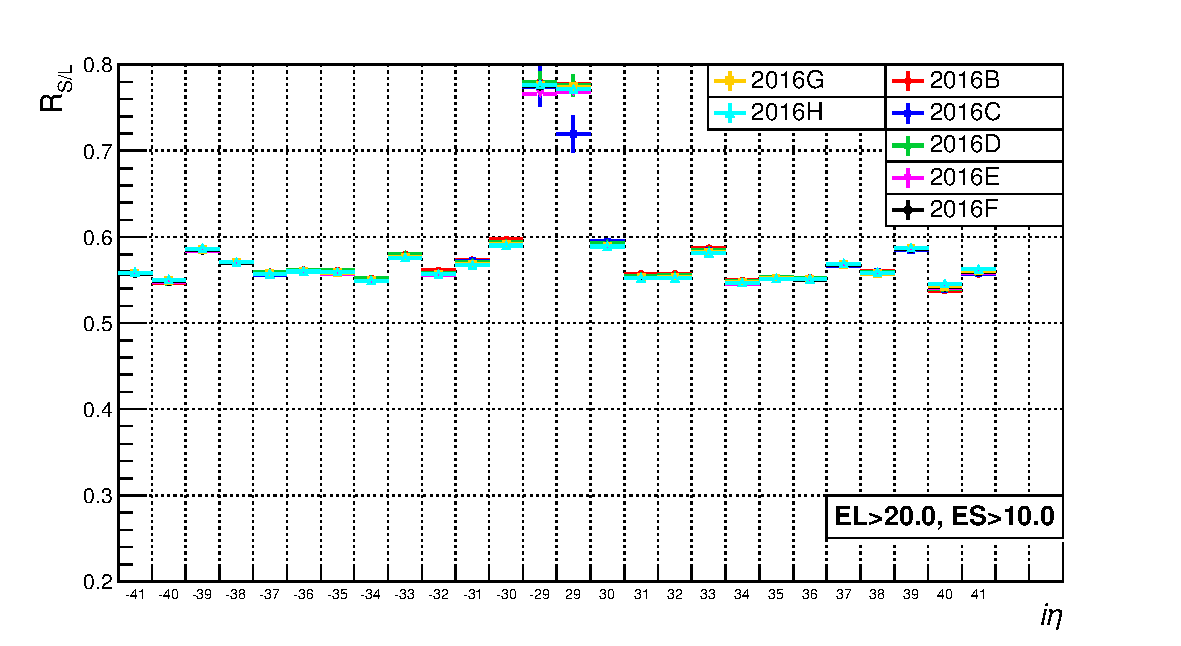
\includegraphics[width=0.8\linewidth]{../Figures/Chap2/ImageFiles_HF/Ratio/2016/RatioVsIeta2016EL20ES10.pdf}
\caption{$\ratiosl$ vs $i\eta$ for 2016 with lower $E_{long}$ threshold}
%\caption{(a)}
\label{RatioVsIeta2016EL20ES10}
%\end{minipage}
\end{figure}
\begin{figure}[h!]%R vs ieta 2016
%\begin{minipage}[c]{0.5\linewidth}
\centering
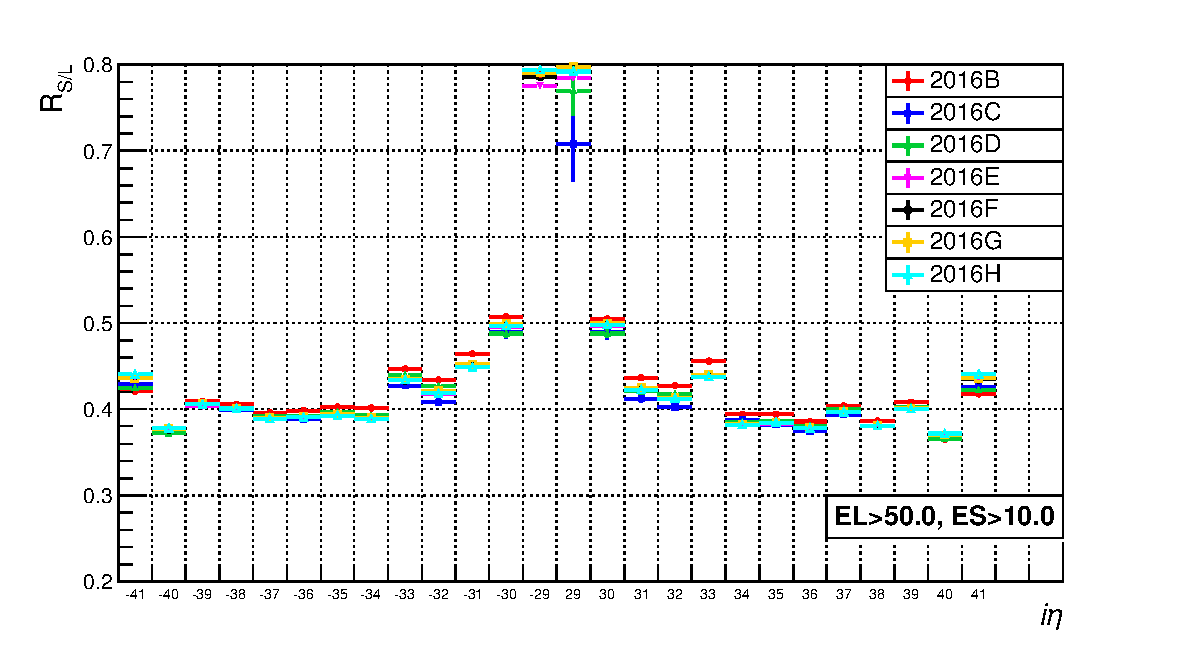
\includegraphics[width=0.8\linewidth]{../Figures/Chap2/ImageFiles_HF/Ratio/2016/RatioVsIeta2016EL50ES10.pdf}
\caption{$\ratiosl$ vs $i\eta$ for 2016 with higher $E_{long}$ threshold}
%\caption{(b)}
\label{RatioVsIeta2016EL50ES10}
%\end{minipage}
%\caption{Mean \ratiosl vs $i\eta$ for 2016 runs with lower (a) and higher (b) $E_{long}$ threshold}
\end{figure}

Corresponding to each $i\eta$ channels, there are 36 divisions in HF. ($|i\eta| = 40,41 $ have 18 divisions). 
\ratiosl as a function of $i\phi$ for a given $i\eta$ channel is also studied and a few such plots are shown
in Fig.\ref{RvsIphiFor2016BtoE} and Fig.\ref{RvsIphiFor2016BFGH}. 
% \textcolor{red}{\ratiosl vs $i\phi$ for all other $i\eta$ are shown in appendix \ref{fig:ieta29_32_E1E2Cut0Ietaiphi2016BtoE} - \ref{fig:ieta41_E1E2Cut0Ietaiphi2016BFGH}.}
Across all the channels for all these run eras, \ratiosl show consistent features. These plots clearly indicate
that \ratiosl is stable across different run eras.\\
To make sure that there is no bias involved in using the JetHT dataset, comparison of \ratiosl for 
JetHT and a dataset consisting of muons (triggered by a muon with $\pt > 50$ \gev)  is done. 
These two datasets showed very similar \ratiosl % \textcolor{red}{and the plot is shown in fig.\ref{fig:2016B2SingMu} appendix A}.
\begin{figure}[!h] %R vs iphi 2016BtoE
\begin{minipage}[c]{0.5\linewidth}
\centering
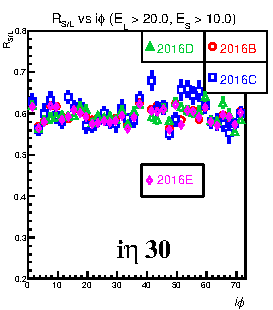
\includegraphics[width=0.7\linewidth]{../Figures/Chap2/ImageFiles_HF/Ratio/2016/ieta30For2016BtoE.pdf}
\end{minipage}
\begin{minipage}[c]{0.5\linewidth}
\centering
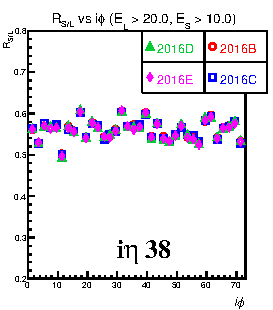
\includegraphics[width=0.7\linewidth]{../Figures/Chap2/ImageFiles_HF/Ratio/2016/ieta38For2016BtoE.pdf}
\end{minipage}
\caption{\ratiosl vs $i\phi$ for 2016B,C,D,E}
\label{RvsIphiFor2016BtoE}
\end{figure}
\begin{figure}[!h] %R vs iphi 2016BFGH
\begin{minipage}[c]{0.5\linewidth}
\centering
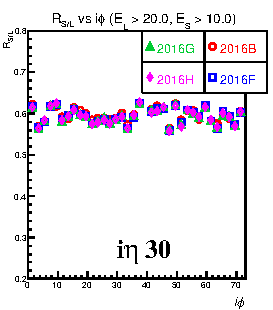
\includegraphics[width=0.7\linewidth]{../Figures/Chap2/ImageFiles_HF/Ratio/2016/ieta30For2016BFGH.pdf}
\end{minipage}
\begin{minipage}[c]{0.5\linewidth}
\centering
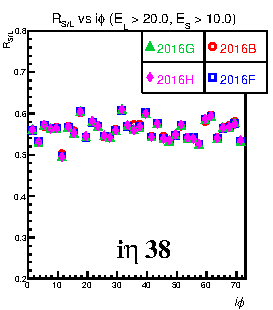
\includegraphics[width=0.7\linewidth]{../Figures/Chap2/ImageFiles_HF/Ratio/2016/ieta38For2016BFGH.pdf}
\end{minipage}
\caption{\ratiosl vs $i\phi$ for 2016B,C,D,E}
\label{RvsIphiFor2016BFGH}
\end{figure}

\subsection{Corrections for the \ratiosl Based on $\phi$ Symmetry}
All the physics processes are symmetric in the azimuthal, $\phi$ direction ( or the transverse x-y plane). 
So \ratiosl is also expected to be symmetric or flat across all $\phi$ channels for a given $\eta$ or $i\eta$.
Based on this symmetry, corrections are derived for the ratio such that \ratiosl is constant across all the $\phi$ channels for a given $\eta$. The corrections are derived as follows:
\begin{itemize}
\item Fit the \ratiosl vs $i\phi$ plot of 2016B with line of 0 slope, and intercept k.
\item Correction for a channel is nothing but original \ratiosl times the intercept.
\end{itemize}
\begin{equation}
Correction(i\eta,i\phi) = k_{i\eta} \times \ratiosl \\
\end{equation}
\begin{equation}
Corrected\ ratio(i\eta,i\phi) = R_{S/L}^{Corr} = Correction(i\eta,i\phi) \times \ratiosl
\end{equation}
These corrections are obtained for all the channels of HF using 2016B dataset with $E_{long} > 50~GeV$ and $E_{Short} > 10~GeV$. The corrections factors as a function of $\eta$ and $i\phi$ are shown in Fig.\ref{fig:corrFacEL50ES10}. 
%These correction factors are also listed in tab.\ref{tab:corrFacPosEta} and tab.\ref{tab:corrFacNegEta} of appendix.
These corrections are applied to 2016B and the remaining 2016 run eras with the same threshold on $E_{long}$ and $E_{Short}$.
 (The errors on the correction factors are dependent on the error on the mean \ratiosl and the fit uncertainty. These errors are less than 1\% for almost all the channels, except for $|i\eta|$=29)
\begin{figure}[h]
\centering
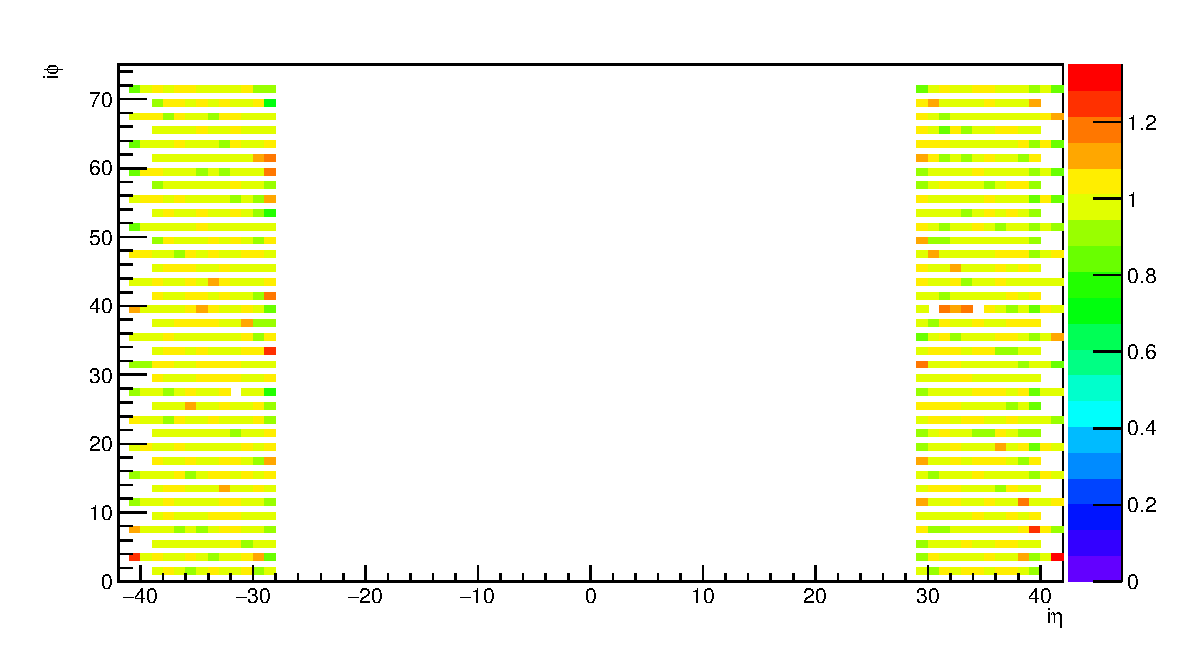
\includegraphics[width=0.7\linewidth]{../Figures/Chap2/ImageFiles_HF/Ratio/2016/corrFacEL50ES10.pdf}
\caption{Correction factors as a function of $i\eta, i\phi$}
\label{fig:corrFacEL50ES10}
\end{figure}

Fig.~\ref{corrected2016BFGH_38} shows the comparison of ratio plots before correction (left)and after correction (right). Similar features are seen for other run eras i.e, 2016C,D and E. %Complete set of plots corresponding to all run eras are shown in appendix Fig.\ref{fig:ieta29_32_E1E2Cut3IetaiphiBtoE} - Fig.\ref{fig:ieta41_E1E2Cut3Ietaiphi_Crrtd}. (2016C and 2016D have low statistics and hence the errors would be large)\\

\begin{figure}[!h] %R corrected vs iphi 2016BFGH
\begin{minipage}[c]{0.5\linewidth}
\centering
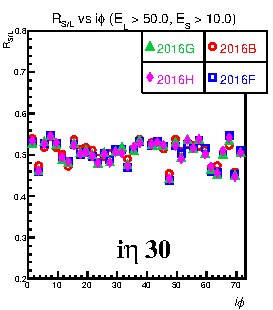
\includegraphics[width=0.7\linewidth]{../Figures/Chap2/ImageFiles_HF/Ratio/2016/Corrected/ieta30Cut3Ietaiphi.pdf}
\end{minipage}
\begin{minipage}[c]{0.5\linewidth}
\centering
\includegraphics[width=0.7\linewidth]{../Figures/Chap2/ImageFiles_HF/Ratio/2016/Corrected/ieta30Cut3Ietaiphi_corr.pdf}
\end{minipage}
\caption[\ratiosl vs $i\phi$ for $i\eta=30$ before and after corrections]{\ratiosl vs $i\phi$ for $i\eta=30$ for (left) current detector, and (right) after corrections for 2016B,F,G,H}
\label{corrected2016BFGH_30}
\end{figure}

\begin{figure}[!h] %R corrected vs iphi 2016BFGH
\begin{minipage}[c]{0.5\linewidth}
\centering
\includegraphics[width=0.7\linewidth]{../Figures/Chap2/ImageFiles_HF/Ratio/2016/Corrected/ieta38Cut3Ietaiphi.pdf}
\end{minipage}
\begin{minipage}[c]{0.5\linewidth}
\centering
\includegraphics[width=0.7\linewidth]{../Figures/Chap2/ImageFiles_HF/Ratio/2016/Corrected/ieta38Cut3Ietaiphi_corr.pdf}
\end{minipage}
\caption[\ratiosl vs $i\phi$ for $i\eta=38$ before and after corrections]{\ratiosl vs $i\phi$ for $i\eta=38$ for (left) current detector, and (right) after corrections for 2016B,F,G,H}
\label{corrected2016BFGH_38}
\end{figure}
Corrections derived so far had energy threshold on long as 50 GeV and almost no energy threshold on short energy (10 GeV). Using 50 GeV threshold on long makes the corrections less prone to pileup dependencies. To check the dependency of the corrections on energy thresholds used, these corrections are also used for the ratio plots with different thresholds on long for the same dataset 2016B. Fig.~\ref{Ecut1CorrectionEcut3} and \ref{Ecut4CorrectionEcut3} show the ratio plots before and after corrections for the energy thresholds $E_{long} > 30~GeV$ and $E_{long} > 100~GeV$. The corrections are derived from 2016B with $E_{long} > 50~GeV$. The corrected points are multiplied by a factor of 1.3 so that they can be visualized in the same plots. %Fig.~\ref{fig:ieta29_32_E1E2Cut1Ietaiphi_Crrtd} - Fig.~\ref{fig:ieta41_E1E2Cut4Ietaiphi_Crrtd} in appendix shows all the plots corresponding to all $i\eta$ channels with these thresholds.
\begin{figure}[!h] %R corrected vs iphi 2016BFGH Energy
\begin{minipage}[c]{0.5\linewidth}
\centering
\includegraphics[width=0.7\linewidth]{../Figures/Chap2/ImageFiles_HF/Ratio/2016/Corrected/EnegyCut3010/ieta30Ecut1CorrectionEcut3.pdf}
\end{minipage}
\begin{minipage}[c]{0.5\linewidth}
\centering
\includegraphics[width=0.7\linewidth]{../Figures/Chap2/ImageFiles_HF/Ratio/2016/Corrected/EnegyCut3010/ieta38Ecut1CorrectionEcut3.pdf}
\end{minipage}
\caption[\ratiosl vs $i\phi$ with $E_{long} > 30$, $E_{short} >10$]{\ratiosl vs $i\phi$ before and after corrections for 2016B with $E_{long} > 30$, $E_{short} >10$}
\label{Ecut1CorrectionEcut3}
\end{figure}
\begin{figure}[!h] %R corrected vs iphi 2016BFGH Enegy
\begin{minipage}[c]{0.5\linewidth}
\centering
\includegraphics[width=0.7\linewidth]{../Figures/Chap2/ImageFiles_HF/Ratio/2016/Corrected/EnergyCut10010/ieta30Ecut4CorrectionEcut3.pdf}
\end{minipage}
\begin{minipage}[c]{0.5\linewidth}
\centering
\includegraphics[width=0.7\linewidth]{../Figures/Chap2/ImageFiles_HF/Ratio/2016/Corrected/EnergyCut10010/ieta38Ecut4CorrectionEcut3.pdf}
\end{minipage}
\caption[\ratiosl vs $i\phi$ with $E_{long} > 100$, $E_{short} >10$]{\ratiosl vs $i\phi$ before and after corrections for 2016B with $E_{long} > 100$, $E_{short} >10$}
\label{Ecut4CorrectionEcut3}
\end{figure}

It is clear from the Fig.\ref{corrected2016BFGH_38}-Fig.\ref{Ecut4CorrectionEcut3} that using the corrections on the ratio, improves the symmetry in $\phi$.\\
The long fibers are be calibrated using $Z\rightarrow e^+ + e^-$ events. The plots shown indicate that \ratiosl is stable across different runs and it improves the $\phi$ symmetry. So \ratiosl can be used as a tool to inter-calibrate the short fibers.


\subsection{Performance of \ratiosl in data \& MC}\label{sec:ana25ns}
In this section comparison of QCD MC sample with data is done. JetHT dataset of 2016E is used for the studies. Trigger used to select events in the data is found to be $\approx 100\%$ efficient for jet $p^T>500~$GeV. There is no trigger requirement for the MC samples. Apart from this selection, the event must contain (in both data and MC) at least one jet with $p^T>600~$GeV and within $|\eta|<2.4$. Nominal HF rechit filters are also used.\\
Data and MC have different number of observed interactions or different pileup (Fig.\ref{fig:DataMCobsIntPUWt}). So MC is re-weighted such that the observed number of interactions in data and MC match. 
Solid blue line corresponds to the observed interactions in MC before PU re-weighting and dotted blue refers to observed interactions in MC after PU re-weighting.\\
MC is scaled to integrated luminosity of the data ($=4.05\ \fbinv$). After this scaling of MC, MC had more events (integral) than data (about 20\% higher). So MC is scaled down so that the integrals in data and MC match. 

\begin{figure}[h!]
\centering
\includegraphics[width=0.7\linewidth]{../Figures/Chap2/ImageFiles_HF/BasicPics/DataMC/DataMCobsIntPUWt}
\captionsetup{width=.9\linewidth}
\caption[Observed no. of interactions in data and MC]{Observed number of interactions in data and MC (Solid blue line- MC before PU re-weighting, dotted blue-after PU re-weighting).}
\label{fig:DataMCobsIntPUWt}
\end{figure}
Fig.~\ref{fig:nVtxDataMC} shows the number of reconstructed primary vertices and Fig.~\ref{fig:nRecHitsDataMC} shows the number of HF rechits above 10 GeV (after all MC re-weightings mentioned above).

\begin{figure}[h!]
\begin{minipage}[c]{0.5\linewidth}
\centering
\includegraphics[width=0.9\linewidth]{../Figures/Chap2/ImageFiles_HF/BasicPics/DataMC/nVtxDataMC}
\captionsetup{width=.9\linewidth}
\caption{Number of reconstructed primary vertices in data and MC}
\label{fig:nVtxDataMC}
\end{minipage}
\begin{minipage}[c]{0.5\linewidth}
\centering
\includegraphics[width=0.9\linewidth]{../Figures/Chap2/ImageFiles_HF/BasicPics/DataMC/nRecHitsDataMC}
\captionsetup{width=.9\linewidth}
\caption{Number of HF rechits above 10 GeV}
\label{fig:nRecHitsDataMC}
\end{minipage}
\end{figure}

\begin{figure}[h!]
%\begin{minipage}[c]{0.32\linewidth}
%\centering
\includegraphics[width=0.32\textwidth]{../Figures/Chap2/ImageFiles_HF/BasicPics/DataMC/HFEnergyDataMC}
%\caption{HF rechit energy distribution}
%\label{fig:HFEnergyDataMC}
%\end{minipage}
%\begin{minipage}[c]{0.329\linewidth}
%\centering
\includegraphics[width=0.32\textwidth]{../Figures/Chap2/ImageFiles_HF/BasicPics/DataMC/ELDataMC}
%\caption{Energy in long(depth1)}
%\label{fig:ELDataMC}
%\end{minipage}
%\begin{minipage}[c]{0.32\linewidth}
%\centering
\includegraphics[width=0.32\textwidth]{../Figures/Chap2/ImageFiles_HF/BasicPics/DataMC/ESDataMC}
\caption[HF rechit energy in data and MC]{Distribution of energies in (left) all HF rechits, (middle) long fibers or depth\,1, and (right) in short fibers or depth\,2.}
%\label{fig:ESDataMC}
%\end{minipage}
\label{fig:HFEnergyDataMC}
\end{figure}

Fig.~\ref{fig:HFEnergyDataMC} (left) shows the energy distribution in HF. The energy distributions in data and MC show different behavior. Fig.~\ref{fig:HFEnergyDataMC} (middle) shows energy in long and fig.\ref{fig:HFEnergyDataMC} (right) shows the energy in short. The energy distributions in long fibers show more discrepancies as compared to the ones in short. In data, energy falls more rapidly than the ones shown by MC.

\subsubsection{$ \ratiosl$ vs $i\eta$}
Average \ratiosl is determined for data and MC with different energy thresholds on $E_{long}$ and $E_{short}$ and they are plotted as a function of $i\eta$ (Fig.~\ref{fig:DataMCRIeta2010} - Fig.~\ref{fig:DataMCRIeta10010}). If the energy threshold is low (Fig.~\ref{fig:DataMCRIeta2010}), data and MC show large discrepancies. If  higher $E_{long}$ threshold is used, then the agreement is better (Fig.~\ref{fig:DataMCRIeta4010}). However increasing the $E_{long}$ threshold to very high values also shows discrepancies (Fig.~\ref{fig:DataMCRIeta10010}). Increasing short energy threshold along with long threshold gives better agreement (Fig.~\ref{fig:DataMCRIeta5050}) between data and MC. The differences are present at long and short energy itself (Fig.~\ref{fig:HFEnergyDataMC}). If data and MC agree for certain thresholds, then it because the differences in long and short cancel to some extent.\\
As the energy thresholds are varied, shape of the distributions in these plots also change. One reason is that, shape of \ratiosl distribution is different for different $i\eta$ (fig.\ref{goodfit} and fig.\ref{badfit}). The other reason is because of the correlation between long and short energies. Any threshold on long or short affects the energy in the other. In fig.\ref{fig:DataMCRIeta5050}, the threshold on long and short are same (50GeV). This energy threshold will not select many of EM showers since $E_{short}$ is very high. In other words, different thresholds select different EM and hadronic components.

\begin{figure}[h!]
\centering
\includegraphics[width=0.6\linewidth]{../Figures/Chap2/ImageFiles_HF/Ratio/DataMC/DataMCRIeta2010}
\caption{\ratiosl vs $|i\eta|$ with $E_{long}>20,E_{short}>10$ GeV}
\label{fig:DataMCRIeta2010}
\end{figure}
\begin{figure}[h!]
\centering
\includegraphics[width=0.6\linewidth]{../Figures/Chap2/ImageFiles_HF/Ratio/DataMC/DataMCRIeta4010}
\caption{\ratiosl vs $|i\eta|$ with $E_{long}>40,E_{short}>10$ GeV}
\label{fig:DataMCRIeta4010}
\end{figure}

\begin{figure}[h!]
\centering
\includegraphics[width=0.6\linewidth]{../Figures/Chap2/ImageFiles_HF/Ratio/DataMC/DataMCRIeta10010}
\caption{\ratiosl vs $i\eta$ with $E_{long}>100,E_{short}>10$}
\label{fig:DataMCRIeta10010}
\end{figure}

\begin{figure}[h!]
\centering
\includegraphics[width=0.6\linewidth]{../Figures/Chap2/ImageFiles_HF/Ratio/DataMC/DataMCRIeta5050}
\caption{\ratiosl vs $i\eta$ with $E_{long}>50,E_{short}>50$}
\label{fig:DataMCRIeta5050}
\end{figure}

\subsubsection{$ \ratiosl$ vs $i\phi$}
Since \ratiosl vs $i\eta$ plots for data and MC show differences, it is obvious that \ratiosl does not agree for different $i\phi$s as well (Fig.~\ref{fig:RatioVsIphiDataMC}). However, it can be seen that \ratiosl is flat (constant across all $i\phi$) for a given $i\eta$.
\begin{figure}[h!]
%\begin{minipage}[c]{0.5\linewidth}
\centering
\includegraphics[width=0.45\linewidth]{../Figures/Chap2/ImageFiles_HF/Ratio/DataMC/ieta30_E1E2Cut3Ietaiphi}
%\caption{}
%\label{fig:ieta30_E1E2Cut3Ietaiphi}
%\end{minipage}
%\begin{minipage}[c]{0.5\linewidth}
%\centering
\includegraphics[width=0.45\linewidth]{../Figures/Chap2/ImageFiles_HF/Ratio/DataMC/ieta38_E1E2Cut3Ietaiphi}
%\caption{}
%\label{fig:ieta38_E1E2Cut3Ietaiphi}
%\end{minipage}
\caption{\ratiosl vs $i\phi$ for data and MC}
\label{fig:RatioVsIphiDataMC}
\end{figure}

\subsection{Summary of HF studies using \ratiosl}
Study of performance of hadron forward (HF) calorimeter was done using ratio of energy deposited in short to long fibers (\ratiosl) of HF. Data collected by CMS in 2012 with $\sqrt{s}=13$TeV was compared with 2015 data using \ratiosl. For most of the $i\eta$ towers, 2012 showed lower \ratiosl than 2015, which might be because of increased $\sqrt{s}$ or radiation damage. Affect of pileup on \ratiosl was studied and with increased pileup, \ratiosl was found to decrease. Comparison of 25ns bunch spacing 2015 data and 2016 data was done and \ratiosl showed similar features. Different run eras of 2016 also showed similar \ratiosl, which indicates the stability of \ratiosl across these run eras. For a given $i\eta$, different $i\phi$s showed small variations in \ratiosl. Corrections were obtained using 2016B to make the \ratiosl constant (flat) across these $\phi$ channels and these corrections improved flatness of \ratiosl. Assuming that long fibers are well calibrated within a given $i\eta$, these corrections can be used intercalibrate short fibers. Comparison of data and MC was also done and these shows differences in terms of energy distribution in long and short fibers. \ratiosl also shows differences for many of the channels. The agreement in terms of \ratiosl is better for higher enrgy threholds.






\section{Trigger system}																			
\begin{wrapfigure}{r}{0.45\linewidth}
\includegraphics[width=0.9\linewidth]{../Figures/Chap2/xsec13TeV_36_SM}
\captionsetup{width=.9\linewidth}
\caption[SM cross section vs SUSY cross section]{Comparison of cross section for various SM processes and SUSY processes.}\label{fig:xsec13TeV_36_SM}
\end{wrapfigure}
In CMS, two levels of triggering system is used to reduce the rate of data flow from various detectors. The first level trigger (L1) is hardware based and the second level is software based (high level or HLT). The trigger system is inevitable since there is several orders of magnitude difference between inelastic pp cross section and other SM and SUSY processes. Figure \ref{fig:xsec13TeV_36_SM} shows the cross section (on left y-axis) for various SM processes, and SUSY processes which are theoretically calculated \cite{Borschensky:2014cia}. Inelastic pp is of no interest to LHC physics and hence these events in pp collision need to be filtered out. There are also limiting factors in terms of the rate of writing into a disk and storage capacity.

The pp collision frequency is 40 MHz. The L1 trigger (L1T) system uses custom hardware made using field programmable gate arrays (FPGAs) and GaAs application-specific integrated circuits (ASICs). The output rate is adjusted depending on the LHC luminosity and it is maintained below 100 kHZ which is the upper limit imposed by readout electronics. It selects events containing various candidate objects or a combination of the objects - ionization deposits consistent with muon, or ECAL energy clusters for electrons/photons, or energy deposits in calorimeters expected from $\tau$, jet, or missing transverse momentum obtained by vectorially summing the objects and using transverse component. A schematic diagram of L1T is shown in Fig.\ref{fig:L1Tsystem} \cite{Khachatryan:2016bia}.
\begin{figure}[h!]
\centering
\includegraphics[width=0.7\linewidth]{../Figures/Chap2/L1Tsystem}
\caption[Schematic of L1T]{A schematic digram of L1T \cite{Khachatryan:2016bia}.}
\label{fig:L1Tsystem}
\end{figure}
The data from calorimeters is processed regionally and globally forming regional and global calorimeter trigger (RCT and GCT). Global muon trigger (GMT) is formed by taking hits from various muon systems by making use of pattern comparator or segment and track finder. The global trigger (GT) makes the final decision about the event by combining GCT and GMT. This decision is sent to CMS subdetectors via trigger timing and control (TTC). The DAQ (data acquisition system) reads data from subsystems for offline processing.

HLT performs reconstruction and identification of objects similar to offline, but faster and less precise. It makes use of several computers which run various algorithms in a predefined order and increasing complexity. Selections based on the information from calorimeters and muon chambers is carried out first and then the CPU intensive tracking reconstruction. The output data flow from HLT is about 400 Hz and it is used for offline storage. 

\section{Object reconstruction}
The identification and reconstruction of various physics objects is done using the information from subdetectors using particle-flow (PF) algorithm \cite{CMS-PRF-14-001}. Fig.\ref{fig:CMS_PF} shows the interaction of different particles in a transverse slice of CMS detector.
\begin{figure}[h!]
\centering
\includegraphics[width=0.95\linewidth]{../Figures/Chap2/CMS_PF}
\caption[Particle interaction in CMS]{A sketch showing interaction of particles in a slice of CMS detector}
\label{fig:CMS_PF}
\end{figure}
The charged particles leave signatures in various layers of the inner tracker because of 3.8 T magnetic filed provided by the solenoid. Muon, being charged and minimum ionizing particle, bends in magnetic field and gives hits in the tracker and outer muon chambers. Electrons give hits in tracker and deposit almost all their energy in the ECAL. Photons can be identified if there is energy deposit in ECAL, but no track. Hadrons deposit most of the energy in HCAL and distinction of neutral and charged hadron is done by the presence of track.

\subsection{Tracking}
Track reconstruction takes place using a combinatorial track finder (CTF) algorithm based on Kalman filtering (KF). Full tracking is an iterative process starting with the easiest tracks and then proceeding to find more difficult tracks. After each iteration, hits compatible with the tracks are removed and this reduces the number of hits to use for the next iteration. There are 4 steps in an iteration.
\begin{itemize}
\item \textbf{Seed generation:} Finding track candidates using 2-3 hits compatible with charged particle trajectory.
\item \textbf{Track finding:} Extrapolate the trajectory of the seeds to find compatible hits in the other layers using KF technique.
\item \textbf{Track fitting:} Perform fitting to smooth the trajectory and find track parameters - origin, \pt and direction.
\item \textbf{Track selection:} Apply selection criteria on the tracks based on number of layers with a hit, number of layers with missing hits, number of 3D hits, goodness of fit ($\chi^2$) and impact parameters of the track.
\end{itemize}
For the next iteration, hits used in this iteration are removed and some of the selection criteria are changed in order to reconstruct more difficult tracks which originate because of missing hits in the pixel detector, particle interactions and decays, high \pt jets with collimated particles etc.

The basic idea in tracking of electrons is extrapolation of tracks to ECAL energy clusters. The iterative tracking mentioned above is efficient for non-radiating electrons. Because of non-negligible tracker material (Fig.\ref{fig:tracker_material}), electrons radiate photons. Depending on the energy of the radiated photon, values of $\chi^2$ and number of hits may vary. In these cases, Gaussian-sum filter (GSF) technique \cite{Adam_2005} is used instead of KF. GSF fitting allows for sudden change in momentum of the tracks as the electron passes through various layers of tracker. Finally, a requirement is applied on the score of a boosted decision tree (BDT) classifier which uses various parameters of the KF and GSF tracks.

\subsection{Interaction vertices}
When the pp bunches collide at the LHC, multiple pp interactions can take place. The goal of vertex reconstruction is to locate the position of such interactions along with the uncertainties associated with it. This process involves 3 steps \cite{Chatrchyan:2014fea}:
\begin{enumerate}
\item selection of tracks: tracks passing quality criteria based on transverse impact parameter relative to the beam spot, number of hits and normalized $\chi^2.$
\item clustering of tracks which seem to originate from same vertex: the $z$-coordinates of the selected tracks measured from center of the beam spot to the point of closest approach are used for clustering. 
The algorithm should be able to resolve very close vertices, but not split a genuine single vertex into many. Deterministic annealing (DA) algorithm \cite{a726788} \cite{Chatrchyan:2014fea} is used for this purpose.
\item fitting the position of each vertex using its associated tracks with the help of adaptive vertex filter \cite{Fruhwirth:2007hz}.
\end{enumerate}
\textcolor{red}{After all interaction vertices are reconstructed, the primary pp interaction vertex is selected as the vertex with the largest $\pt^2$ sum of all physics objects. The physics objects used in this calculation are produced by a jet-finding algorithm ~\cite{Cacciari:2008gp,Cacciari:2011ma} applied to all charged-particle tracks associated to the vertex, plus the corresponding \ptmiss computed from those jets.}

\subsection{Muons}
Since the calorimeters absorb energy of EM objects and hadrons, hits in muon spectrometer can be used to reconstruct muons. These muons which are reconstructed using muon systems only are called \textit{standalone muons}.

If the standalone muon track is compatible with the track from the inner tracker, a new \textit{global muon} track is fitted to the hits from both the systems. 

If at least one muon segment matches with the extrapolated track from inner tracker, corresponding muon is called \textit{tracker muon}. 

The performance of global muon is better than standalone or tracker muon since it uses information from inner tracker and muon system.

The momentum of muon is determined using \textit{Tune-P} algorithm \cite{Chatrchyan:2012xi}. The reconstructed muons are fed into PF algorithm which combines information from other subdetectors of CMS and applies various quality criteria. The identification of muons uses criteria on track fit $\chi^2$, number of hits in tracker or muon chambers or both, compatibility of tracker tracks and hits/tracks in muon chambers and also the  compatibility with primary vertex. Detailed muon reconstruction procedure and its performance in 2015 and 2016 data is described in ref. \cite{Sirunyan:2018fpa}.

\subsection{Electrons and photons}
Electrons and photons interact in similar way in ECAL. The material in the tracker lead to conversion of photons in to $e^+e^-$ pairs and electrons can emit bremsstrahlung photons, photons again convert etc.

When an electron radiates photon, energy is spread in $\phi$ direction because of the magnetic field and negligible spread in $\eta$ direction. The amount of energy radiated depends on $\eta$ and it varies from 33\% to 86\% \cite{Khachatryan:2015hwa}.

An electron candidate is seeded from a GSF track, provided the corresponding ECAL cluster is not linked to 3 or more additional tracks. A photon candidate is seeded from a ECAL energy cluster with transverse energy, $\et > 10\ \gev$ with no link to GSF track.

Two algorithms, \textit{hybdrid} for the barrel (EB) and \textit{multi 5x5} for endcap (EE) \cite{Khachatryan:2015hwa} are used to collect the energy of the radiated photons in case of electron reconstruction or converted photons in case of photon reconstruction. Clustering is performed  on intercalibrated, reconstructed signal amplitudes after taking care of several detector effects. Clustering starts with a seed crystal which is the highest \et crystal in its neighborhood. In EB, clusters are centered on the seed crystal and have a fixed width of 5 crystals in $\eta$. In the $\phi$ direction, adjacent strips of 5 crystals are added. Further $\eta$ aligned crystals may be seeded and added if they lie within $\phi$ window of $\pm17$ crystals. At each step of clustering, predefined thresholds on energy are applied. Clustering in EE is carried out using fixed 5x5 crystal matrices. After identifying the seed crystal, more matrices are added if their centroid lies in  $\eta$ of 0.07 and $\phi$ distance of about 0.3 radians. These matrices are partially allowed to overlap. If the photons do not convert, then superclusters resulting from these algorithms are simply 5x5 matrices. More details about electron and photon reconstruction and performance can be found in ref. \cite{Khachatryan:2015hwa,CMS:EGM-14-001}.

\subsubsection{Photon Identification}
\label{sec:photonID}
The collection of photons derived from PF algorithm have very loose criteria on their properties. For the purpose of analyses, more tighter requirements are placed on photons. The main idea is to get highest efficiency for prompt isolated photons and reject non-prompt photons which are coming from $\pi^0$ decays or part of hadronization process. Several properties of PF photons are studied to distinguish prompt and non-prompt photons. Prompt photons generally have smaller energy spread in ECAL and very less energy deposit in HCAL. Non-prompt photons are associated with charged or neutral hadrons nearby and they deposit energy in HCAL and sometimes a part of their energy in ECAL leading to larger ECAL clusters. Table \ref{tab:photonID} shows a list of variables and their values used for selecting photons in this SUSY search.
\begin{table}[h!]
\centering
\captionsetup{width=.99\linewidth}
\caption[Photon Identification ]{A list of variables used for identification (ID) of photons in barrel and endcap. Prompt photon properties should not exceed any of the values listed in this table. Bottom 2 rows show the efficiency for signal (prompt photons) and background (non-prompt photons).}
\label{tab:photonID}
\begin{tabular}{c|c|c}
\hline
Property		&	Max value in EB		&	Max value in EE\\\hline\hline
H/E					&	0.05				&	0.05\\
$\sigma_{i\eta i\eta}$&	0.0102				&	0.0274\\
PF $h^\pm$ iso	&	3.32		&	1.97\\
PF $h^0$ iso	&	$1.92 + 0.014\pt + 0.000019\pt^2$	&	$11.86 + 0.0139\pt+0.000025\pt^2$\\
PF $\gamma$ iso	&	$0.81 + 0.0053\pt$	&	$0.83 + 0.0034\pt$\\\hline\hline
Efficiency		&	EB (\%)			&	EE (\%) \\\hline
Signal			&	90					&	90 \\
Background		&	16					&	18\\\hline
\end{tabular}
\end{table}
Description of variables used for photon identification:
\begin{itemize}
\item H/E: Ration of energy in HCAL tower behind ECAL supercluster to energy of supercluster.
\item $\sigma_{i\eta i\eta}$: This is a shower shape variable which is the second moment of the energy distribution along the $\eta$ coordinate.
\begin{equation}
\sigma_{i\eta i\eta}^2 = \frac{\sum\limits_{i}^{5\times5}w_i(i\eta_i-i\eta_{seed})^2}{\sum\limits_{i}^{5\times5}w_i}, \hspace{1cm}
w_i = max(0,\ 4.7+\ln\frac{E_i}{E_{5\times5}})
\end{equation}
The summation runs over 5x5 crystal matrix around most energetic crystal in the supercluster.
\item PF $h^\pm$ iso: PF charged hadron isolation variable which is defined as sum of \pt of all PF charged hadrons which are
associated to the primary vertex, not in the footprint of the candidate photon, and within a cone of \dR = 0.3.
\item PF $h^0$ iso: Pileup corrected PF neutral hadron isolation defined as sum of \et of all PF neutral hadrons which are not in the footprint of the candidate photon and are within a cone of \dR = 0.3.
\item PF $\gamma$ iso: Pileup corrected PF photon or $\gamma$ isolation is defined as sum of \et of all PF photons which are not in the foot-print of
the candidate photon and are within a cone of \dR = 0.3.
\end{itemize}
The PF $h^0$ and $\gamma$ isolations are corrected for pileup contributions using $\mathrm{Iso}_{\mathrm{corr}} = \mathrm{Iso}_{\mathrm{original}} - \rho\mathrm{EA}$, where $\rho$ is the energy density of the event calculated using FastJet package \cite{Cacciari:2011ma} which is a measure of pileup activity in the event per unit area and EA is the effective area.

To reject mis-identification of electrons into photons, an additional criteria called \textit{pixel seed veto} is also used. If the ECAL energy cluster is associated with hit(s) in the pixel detector then the corresponding electron or photon is said to have pixel seed. 

This identification criteria shown in table \ref{tab:photonID} with pixel seed veto is called \textit{loose ID + pixel seed veto}. The efficiency for this selection in shown in figure \ref{fig:PhotonEfficiencies}. This efficiency is determined using simulation with data to simulation corrections applied.
\begin{figure}[h!]
\centering
\includegraphics[width=0.7\linewidth]{../Figures/Chap2/PhotonEfficiencies}
\captionsetup{width=.99\linewidth}
\caption[Loose + pixel seed veto photon efficiency]{Efficiency for loose ID + pixel seed veto photons determined from simulation. The uncertainty includes statistical and systematic.}
\label{fig:PhotonEfficiencies}
\end{figure}

\subsubsection{Electron Identification}
\label{sec:eleID}
Various quality criteria are applied to PF electrons in a similar way as photons. Since electron also has a track, electron ID makes use of track based variables apart from photon ID variables. In this analysis, we use \textit{mini-isolation, $I_{mini}<0.1$} instead of isolation calculated using fixed cone size of $\dR$ = 0.3.
\begin{equation}
I_{mini} = \frac{\sum_{R}^{}\pt (h^\pm) + max(0,\sum_{R}^{}\pt(h^0)+\pt(\gamma) - \rho EA (\frac{R}{0.3})^2)}{\pt (e)}
\end{equation}
The variables used in this equation are same as the ones used for photon and its calculation is similar to the way as fixed cone isolation is calculated, except that the isolation cone size is dependent on \pt of the electron \cite{Rehermann:2010vq}. The size of the cone varies as:
\[
R = \left\{
\begin{array}{ll}
0.2\ &\mathrm{if\ \pt < 50\ \gev}\\
10\ \gev /\pt &\mathrm{if\ 50 < \pt < 200\ \gev}\\
0.05 &\mathrm{if\ \pt > 200\ \gev}	
\end{array}
\right.
\]
In case of boosted $t\bar{t}$ events involving $W\to e\nu$, b-jet from top decay may be very close to electron. The fixed cone isolation becomes inefficient in identifying these kind of electrons. Since the cone size is smaller for large \pt electrons in case of mini-isolation, the efficiency for identification of such electrons is high with mini-isolation.

The efficiency of mini-isolation (or any other identification criteria) can be measured using \textit{tag \& probe} (TnP) technique both in data and MC. If there are differences in data and MC efficiencies, corrections are applied to MC and these corrections are called as scale factors (SFs). Tag object is a well identified electron with very strict criteria on its properties. This object needs to have \pt $>30$ \gev and $|\eta|<2.17$ and matched with any of the electron HLT trigger objects ($\dR(\mathrm{Tag,\ HLT\ object})<0.3$). Probe object is the electron whose efficiency needs to be measured and it has charge opposite to that of tag. To calculate the efficiency of any isolation, we also impose the condition on probe that it passes an ID criteria which does not use isolation variables. In this case we have applied a multivariate technique based electron identification criteria on the probes. The decay of Z boson gives a pair of electrons and one the electrons serves as tag and the other as probe. By using the 4-momenta of electrons, invariant mass of Z boson can be reconstructed. Figure \ref{fig:bin25_el_sc_eta_0p00To0p80_el_pt_35p00To50p00} shows the invariant mass distribution of tag and probe pairs in data collected in 2016 for events with probe $\pt \in 35 - 50\ \gev$ and $\eta < 0.8$. The left plot corresponds to events in which probe object passes min-isolation criteria and right plot corresponds to events in which probe fails mini-isolation criteria. 
\begin{figure}[h!]
\centering
\includegraphics[width=0.9\linewidth]{../Figures/Chap2/bin25_el_sc_eta_0p00To0p80_el_pt_35p00To50p00}
\captionsetup{width=.9\linewidth}
\caption[TnP fit for MiniIso pass/fail]{The left (right) plot shows the invariant mass distribution of tag and probe passing (failing) mini-isolation criteria.}
\label{fig:bin25_el_sc_eta_0p00To0p80_el_pt_35p00To50p00}
\end{figure}
This distribution is fitted with a signal function - MC template with Gaussian smearing shown in red, and a background function - CMS shape function shown in blue. The CMS shape function is a product of falling exponential and error function \cite{Meyer:2239058}. The efficiency is given by the ratio of number events with passing probe to the total number of events with passing/failing probe. This can be determined by taking the area under the signal function from both of the fits. The efficiency for the above figure is found to be 0.97 with negligible statistical uncertainty. The efficiency in MC can be obtained by using the template or using generator level information.

The whole procedure can be repeated by taking other $\pt-\eta$ ranges and calculate the efficiency. To evaluate the systematic uncertainty, refitting is done using different signal function (Crystal-Ball with Gaussian smear) and background function (exponential). Systematic uncertainty because of the choice of tag is evaluated by making a different tag selection. Figure \ref{fig:MiniIsoSF} shows the efficiency (top panel) and SFs (bottom panel) for various $\eta$ regions as a function of \pt.
\begin{figure}[h!]
\centering
\includegraphics[width=0.6\linewidth]{../Figures/Chap2/MiniIsoSF}
\captionsetup{width=.9\linewidth}
\caption[Mini-isolation efficiency and SF]{The efficiency of mini-isolation in data (top panel) as a function of electron \pt for various $\eta$ regions and the bottom panel shows the SFs. The error bars include systematic and statistical uncertainties.}
\label{fig:MiniIsoSF}
\end{figure}

These SFs account for any discrepancies in data and MC and they are applied on MC. In a similar way the SFs are derived to account for discrepancies at track reconstruction level, identification, and isolation (as mentioned here for mini-isolation). Wherever needed, these type of corrections are applied to other physics objects as well. 

 

\subsection{Jets}
Hadronization of quarks and gluons results in formation of many mesons and baryons which is referred to as a jet, deposits its energy mostly in HCAL. On an average 65\% of the total energy of the jet is carried by charged hadrons, 25\% by photons and 10\% neutral hadrons. Figure \ref{fig:JetEfrac} shows the jet energy fraction as a function of \pt in data and simulation. The lower panel shows the difference in data and simulation.
\begin{figure}[h!]
\centering
\includegraphics[width=0.5\linewidth]{../Figures/Chap2/JetEfrac}
\caption[Energy energy composition]{Energy composition in jets as a function of jet \pt in data and MC simulation \cite{CMS-PRF-14-001}.}
\label{fig:JetEfrac}
\end{figure}

Jets are reconstructed using PF candidates using anti-$k_T$ algorithm \cite{Cacciari:2008gp,Cacciari:2011ma} with a size parameter of 0.4. These jets are called as AK4PF jets. They are also subject to pileup mitigation using charged hadron subtraction (CHS). In CHS, charged hadrons associated to vertices apart from primary vertex are removed from PF candidates. To remove remaining energy due to charged hadrons and neutral hadrons, jet area based pileup corrections are applied on an event by event basis. The distance parameters used in jet clustering are:
\begin{align}
d_{ij} &= \mathrm{min}(p_{Ti}^{2n},\  p_{Tj}^{2n})\ (\Delta_{ij}^2/R^2)\\
d_{iB} &= p_{Ti}^{2n}\ \\ 
\mathrm{where\ } \Delta_{ij}^2 &= (y_i-y_j)^2 + (\phi_i - \phi_j)^2
\end{align}
The values of $R$ and $n$ for AK4 jets are 0.4 and -1 respectively. $d_{ij}$ is the distance between entities (particles or psudojets) $i$ and $j$, $d_{iB}$ is the distance between $i$ and the beam (B), $y_i$ is rapidity and $\phi_i$ is the azimuthal angle of $i$th particle. The jet clustering proceeds iteratively by combining \textit{nearest} particles. In the case of anti-$k_T$, the $d_{ij}$ between similarly separated soft particles is higher than the $d_{ij}$ between a hard particle and soft particle. The soft particles in this algorithm do not modify the shape of the jet, but the hard ones do.

The measured energy or the \pt of the jet needs to be corrected so that its measured 4-momentum is close to parton level 4-momentum. There are several reasons for imperfect measurement of jet energy such as pileup energy contribution, non-uniformity of detector response to different jet energy etc. The jet energy corrections (JECs) aim to correct the jets and determine the momentum of the initial parton.
\begin{figure}[h!]
\centering
\includegraphics[width=0.95\linewidth]{../Figures/Chap2/JEC_application}
\captionsetup{width=.95\linewidth}
\caption[Application of JEC]{Pictorial representation of various steps in application of JECs on data and MC simulation \cite{Khachatryan:2016kdb}.}
\label{fig:JEC_application}
\end{figure}
The corrections are derived at different levels (L1, L2 and L3) and the output of each level becomes the input for the other, in other words a factorized approach is followed for applying the corrections. Figure \ref{fig:JEC_application} shows a pictorial representation of different steps in applying JECs both on data and MC simulation. The corrected 4-momenta of the jet can be written as \cite{Chatrchyan:2011ds}:
\begin{align}
p_{\mu}^{corr} &= \mathcal{C}p_{\mu}^{raw}\\
\mathrm{where\ }\mathcal{C} &=C_{\mathrm{offset}}(p_{T}^{raw})\cdot C_{MC}(p_{T}^{\prime},\eta) \cdot C_{rel}(\eta) \cdot C_{abs}(p_{T}^{\prime\prime})
\end{align}
The offset correction, $C_{\mathrm{offset}}$ removes extra energy due to pileup and noise, MC calibration factor, $C_{MC}$ removes bulk of non-uniformity in $\eta$ and non-linearity in \pt, $C_{rel}$ and $C_{abs}$ are relative and absolute energy scale corrections which account for small differences in data and MC. In the expression for $\mathcal{C}$, $p_{T}^{\prime}$ is the \pt of the jet after offset correction, $p_{T}^{\prime\prime}$ is the \pt of the jet after all previous corrections. Figure \ref{fig:JetResp_JECs} shows the average jet \pt response with and without corrections at a few stages of JEC application. The \pt response is defined as the average value of ratio of measured jet \pt to particle-level jet \pt, $p_{T,\mathrm{ptcl}}$.
\begin{figure}[h!]
\centering
\includegraphics[width=0.95\linewidth]{../Figures/Chap2/JetResp_JECs}
\captionsetup{width=.98\linewidth}
\caption[Jet \pt response with and w/o corrections]{Average jet \pt response in QCD MC at different stages of JECs. The left plot is without any corrections, middle plot is for after pileup offset corrections and the right plot is after applying all the JECs. $\mu$ refers to the average number of pileup interactions per bunch crossing.}
\label{fig:JetResp_JECs}
\end{figure}

The resolution of AK4PF jet as a function of ref jet is shown in \ref{fig:JER_2016}. The uncertainty in the jet energy correction is about 2\% for barrel region jets with \pt of 30 \gev \cite{CMS-DP-2018-028}.
\begin{figure}[h!]
\centering
\includegraphics[width=0.8\linewidth]{../Figures/Chap2/JER_2016}
\captionsetup{width=.9\linewidth}
\caption[AK4PF jet energy resolution]{Resolution of PF jets as a function of \pt in the barrel and endcap regions \cite{CMS-DP-2016-020}.}
\label{fig:JER_2016}
\end{figure}
\subsection{Tagging of b-quark jet}
The mass of b-quark is about 4.2 \gev and the hadrons formed from b-quark have masses of 5-6 \gev. The lifetime, $\tau$ of b-hadrons is about 1.5 ps and this corresponds to $c\tau$ value of 0.45 mm. If the momentum of b-hadron is about 200 \gev, the mean decay length is about 2 cm in the lab frame and this increase in decay length is because of Lorentz-boost. With the high position resolution of tracker, it is possible to identify such decays which take place away from the primary vertex (PV). These decay vertices are called secondary vertices and the impact parameter (IP) for such decays is high. In many cases, b-hadron decays result in a soft lepton. Figure \ref{fig:bJet} illustrates a b-jet containing a soft lepton and a secondary vertex (SV).
\begin{figure}[h!]
\centering
\includegraphics[width=0.7\linewidth]{../Figures/Chap2/bJet}
\caption[b-jet showing b-hadron decays]{Illustration of a b-jet showing the decay of a b-hadron and a soft lepton inside the jet \cite{BTV-16-002}.}
\label{fig:bJet}
\end{figure}

The algorithm used for identifying whether a jet is b-jet or not, is called combined SV version-2 (CSVv2) algorithm \cite{BTV-16-002} which combines information about the displaced tracks and the SVs associated with a jet using a multivariate technique. The output of the CSVv2 algorithm is shown in figure \ref{fig:bTagCSVv2op} (left) for u, d, s or gluon jets, c-jets and b-jets in simulated $t\bar{t}$ events. A neural network based CSVv2 tagger (DeepCSV) is also used by CMS. 

The plot on the right side of figure \ref{fig:bTagCSVv2op} shows the efficiency for b-tagging using CSVv2 and DeepCSV as a function of particle-level jet \pt. These efficiencies are obtained from simulation after applying data to simulation corrections. The b-tagged jets (or b-jets) used in this search use CSVv2 - medium working point which has a 55\% efficiency to correctly identify b-jets with $\pt \approx 30$ \gev. The corresponding misidentification probabilities are 1.6\% for gluon and light-flavor quark jets, and 12\% for charm quark jets. 

The efficiency of b-tagging is low at low \pt because of multiple Coulomb interactions and lower Lorentz-boost making the SV closer to PV. At high jet \pt, tracks in the jets are collimated and the curvature of the tracks are small which may cause close-by tracks to create overlapping hits in the tracker.
\begin{figure}[h!]
\centering
\includegraphics[width=0.44\linewidth]{../Figures/Chap2/bTagCSVv2op}
\includegraphics[width=0.52\linewidth]{../Figures/Chap2/btag_eff_CSVv2_DeepCSV}
\captionsetup{width=.98\linewidth}
\caption[CSVv2 output and b-tagging efficiency]{The output of the CSVv2 algorithm for different flavor jets (left) \cite{BTV-16-002}. The right plot shows the efficiency of b-tagging for CSVv2 and DeepCSV as a function of particle-level jet \pt \cite{btagEffTwiki}.}
\label{fig:bTagCSVv2op}
\end{figure}
\subsection{Missing transverse momentum}
The pp collision takes place in $z$ direction and hence the momentum before the collision in $x$ and $y$ directions, transverse direction, is zero. From momentum conservation, final momentum after the collision in transverse direction should be zero. In CMS, PF algorithm is used to reconstruct various particles, except the neutrinos, and these reconstructed particles are called as PF candidates. If there are $n$ PF candidates each of them having a transverse momentum vector $\overrightarrow{p_{T}}$, and a neutrino with transverse momentum vector $\overrightarrow{p_{T}}^{\nu}$, we have
\begin{align}
0 &= \sum_{i}^{\mathrm{n}}\vec{p_{T}}^{i} + \vec{p_{T}}^{\nu} \\
\vec{p_{T}}^{\nu} &= - \sum_{i}^{\mathrm{n}}\vec{p_{T}}^{i}\\
\ptmiss &= |\vec{p_{T}}^{\nu}| = \left|- \sum_{i}^{\mathrm{n}}\vec{p_{T}}^{i}\right|
\end{align}
The transverse momentum of neutrino, $\vec{p_{T}}^{\nu}$ is nothing but the negative vector sum of all PF candidates. Magnitude of this vector is referred to as \ptmiss and it gives the exact \pt of neutrino if we detect and reconstruct all other particles and measure their transverse meomentum accurately. If there are multiple neutrinos or new particles which do not interact with detector, then their momenta get added vectorially and the resulting vector behaves in the same way as $\vec{p_{T}}^{\nu}$, in the context of above equations.
\begin{figure}[h!]
\centering
\includegraphics[width=0.9\linewidth]{../Figures/Chap2/METresoln}
\caption[\ptmiss resolution]{Relative \ptmiss resolution (left) and \ptmiss-$\phi$ resolution as a function of $p_{T,\ \mathrm{ref}}^{miss}$ in simulated $t\bar{t}$ sample \cite{CMS-PRF-14-001}.}
\label{fig:METresoln}
\end{figure}
If PF algorithm is not able to reconstruct and get accurate measurement of momenta all the particles, either because of detector imperfections or finite resolution while measuring momenta of various objects, we get incorrect measure of \ptmiss. The amount of \textit{incorrectness} is termed as fake \ptmiss. As discussed, earlier, jets need various types of corrections to estimate their true 4-momenta. Once the jets are corrected, these corrections need to be propagated to \ptmiss since corrections on jets do not affect PF candidates. The corrected \ptmiss is given by
\begin{equation}
\vec{p_{T}}^{miss,\ corr} = \vec{p_{T}}^{miss} - \sum_{jets}^{}(\vec{p}_{T,jet}^{corr} - \vec{p}_{T,jet}) 
\end{equation}
This \ptmiss is called \textit{type1 corrected \ptmiss} and it uses all jets with $\pt > 15\ \gev$ and having ECAL energy not more than 90\% of the total jet energy. If there is a muon in the jet, then 4-momenta of the muon is subtracted from the jet, corrections are applied, 4-momenta of muon is added back to the corrected jet \cite{CMS-PAS-JME-16-004}.
All the physics objects, electrons, muons, photons, muons and jets (to large extent), play a role in resolution of \ptmiss. Figure \ref{fig:METresoln} shows the relative resolution of \ptmiss (left)and \ptmiss-$\phi$ (right) as a function of $p_{T,\ \mathrm{ref}}^{miss}$, where $p_{T,\ \mathrm{ref}}^{miss}$ is calculated using all stable particles, except neutrinos, from the event generator \cite{CMS-PRF-14-001}.


